\documentclass[twoside]{book}

% Packages required by doxygen
\usepackage{fixltx2e}
\usepackage{calc}
\usepackage{doxygen}
\usepackage[export]{adjustbox} % also loads graphicx
\usepackage{graphicx}
\usepackage[utf8]{inputenc}
\usepackage{makeidx}
\usepackage{multicol}
\usepackage{multirow}
\PassOptionsToPackage{warn}{textcomp}
\usepackage{textcomp}
\usepackage[nointegrals]{wasysym}
\usepackage[table]{xcolor}

% Font selection
\usepackage[T1]{fontenc}
\usepackage[scaled=.90]{helvet}
\usepackage{courier}
\usepackage{amssymb}
\usepackage{sectsty}
\renewcommand{\familydefault}{\sfdefault}
\allsectionsfont{%
  \fontseries{bc}\selectfont%
  \color{darkgray}%
}
\renewcommand{\DoxyLabelFont}{%
  \fontseries{bc}\selectfont%
  \color{darkgray}%
}
\newcommand{\+}{\discretionary{\mbox{\scriptsize$\hookleftarrow$}}{}{}}

% Page & text layout
\usepackage{geometry}
\geometry{%
  a4paper,%
  top=2.5cm,%
  bottom=2.5cm,%
  left=2.5cm,%
  right=2.5cm%
}
\tolerance=750
\hfuzz=15pt
\hbadness=750
\setlength{\emergencystretch}{15pt}
\setlength{\parindent}{0cm}
\setlength{\parskip}{3ex plus 2ex minus 2ex}
\makeatletter
\renewcommand{\paragraph}{%
  \@startsection{paragraph}{4}{0ex}{-1.0ex}{1.0ex}{%
    \normalfont\normalsize\bfseries\SS@parafont%
  }%
}
\renewcommand{\subparagraph}{%
  \@startsection{subparagraph}{5}{0ex}{-1.0ex}{1.0ex}{%
    \normalfont\normalsize\bfseries\SS@subparafont%
  }%
}
\makeatother

% Headers & footers
\usepackage{fancyhdr}
\pagestyle{fancyplain}
\fancyhead[LE]{\fancyplain{}{\bfseries\thepage}}
\fancyhead[CE]{\fancyplain{}{}}
\fancyhead[RE]{\fancyplain{}{\bfseries\leftmark}}
\fancyhead[LO]{\fancyplain{}{\bfseries\rightmark}}
\fancyhead[CO]{\fancyplain{}{}}
\fancyhead[RO]{\fancyplain{}{\bfseries\thepage}}
\fancyfoot[LE]{\fancyplain{}{}}
\fancyfoot[CE]{\fancyplain{}{}}
\fancyfoot[RE]{\fancyplain{}{\bfseries\scriptsize Generated by Doxygen }}
\fancyfoot[LO]{\fancyplain{}{\bfseries\scriptsize Generated by Doxygen }}
\fancyfoot[CO]{\fancyplain{}{}}
\fancyfoot[RO]{\fancyplain{}{}}
\renewcommand{\footrulewidth}{0.4pt}
\renewcommand{\chaptermark}[1]{%
  \markboth{#1}{}%
}
\renewcommand{\sectionmark}[1]{%
  \markright{\thesection\ #1}%
}

% Indices & bibliography
\usepackage{natbib}
\usepackage[titles]{tocloft}
\setcounter{tocdepth}{3}
\setcounter{secnumdepth}{5}
\makeindex

% Hyperlinks (required, but should be loaded last)
\usepackage{ifpdf}
\ifpdf
  \usepackage[pdftex,pagebackref=true]{hyperref}
\else
  \usepackage[ps2pdf,pagebackref=true]{hyperref}
\fi
\hypersetup{%
  colorlinks=true,%
  linkcolor=blue,%
  citecolor=blue,%
  unicode%
}

% Custom commands
\newcommand{\clearemptydoublepage}{%
  \newpage{\pagestyle{empty}\cleardoublepage}%
}

\usepackage{caption}
\captionsetup{labelsep=space,justification=centering,font={bf},singlelinecheck=off,skip=4pt,position=top}

%===== C O N T E N T S =====

\begin{document}

% Titlepage & ToC
\hypersetup{pageanchor=false,
             bookmarksnumbered=true,
             pdfencoding=unicode
            }
\pagenumbering{roman}
\begin{titlepage}
\vspace*{7cm}
\begin{center}%
{\Large Too\+Automation }\\
\vspace*{1cm}
{\large Generated by Doxygen 1.8.11}\\
\end{center}
\end{titlepage}
\clearemptydoublepage
\tableofcontents
\clearemptydoublepage
\pagenumbering{arabic}
\hypersetup{pageanchor=true}

%--- Begin generated contents ---
\chapter{Too\+Automation}
\label{index}\hypertarget{index}{}\href{https://bestpractices.coreinfrastructure.org/projects/1099}{\tt } \href{https://codeclimate.com/github/TaaviE/TooAutomation}{\tt }

This is an easy-\/to-\/use home automation framework at the moment for A\+VR Arduinos with n\+R\+F24\+L01+ radios. A\+RM and P\+IC platform support and 868\+Mhz, 443\+Mhz and Zig\+Bee radio support is planned. 
\chapter{C\+O\+N\+T\+R\+I\+B\+U\+T\+I\+NG}
\label{md_CONTRIBUTING}
\hypertarget{md_CONTRIBUTING}{}
Just try to follow the style that the rest of the code is using. Spaces, not tabs. 
\chapter{Too\+Networking}
\label{md_modules_TooNetworking_README}
\hypertarget{md_modules_TooNetworking_README}{}
A networking library for Too\+Automation. Requires modified version of \href{https://github.com/Avamander/RF24Network}{\tt R\+F24\+Network} to function. 
\chapter{Too\+Signing}
\label{md_modules_TooSigning_README}
\hypertarget{md_modules_TooSigning_README}{}
A signing library for Too\+Automation. Requires modified version of \href{https://github.com/Avamander/RF24Network}{\tt R\+F24\+Network} to function and \href{https://github.com/Cathedrow/Cryptosuite}{\tt A\+T\+S\+H\+A204} library that provides the necessary cryptographic functions. 
\chapter{Module Index}
\section{Modules}
Here is a list of all modules\+:\begin{DoxyCompactList}
\item \contentsline{section}{Reserved message header types by Too\+Networking}{\pageref{group__RESERVED__TYPES}}{}
\end{DoxyCompactList}

\chapter{Class Index}
\section{Class List}
Here are the classes, structs, unions and interfaces with brief descriptions\+:\begin{DoxyCompactList}
\item\contentsline{section}{\hyperlink{union__buffer}{\+\_\+buffer} }{\pageref{union__buffer}}{}
\item\contentsline{section}{\hyperlink{union__state}{\+\_\+state} }{\pageref{union__state}}{}
\item\contentsline{section}{\hyperlink{classATSHA204Class}{A\+T\+S\+H\+A204\+Class} }{\pageref{classATSHA204Class}}{}
\item\contentsline{section}{\hyperlink{structBufferItem}{Buffer\+Item} }{\pageref{structBufferItem}}{}
\item\contentsline{section}{\hyperlink{structNoncePayload}{Nonce\+Payload} }{\pageref{structNoncePayload}}{}
\item\contentsline{section}{\hyperlink{structNonceReceived}{Nonce\+Received} }{\pageref{structNonceReceived}}{}
\item\contentsline{section}{\hyperlink{structNonceRequested}{Nonce\+Requested} }{\pageref{structNonceRequested}}{}
\item\contentsline{section}{\hyperlink{structNonceSent}{Nonce\+Sent} }{\pageref{structNonceSent}}{}
\item\contentsline{section}{\hyperlink{structPayload__Metadata__Received}{Payload\+\_\+\+Metadata\+\_\+\+Received} }{\pageref{structPayload__Metadata__Received}}{}
\item\contentsline{section}{\hyperlink{structPayload__MetadataSigned__Received}{Payload\+\_\+\+Metadata\+Signed\+\_\+\+Received} }{\pageref{structPayload__MetadataSigned__Received}}{}
\item\contentsline{section}{\hyperlink{classSha256Class}{Sha256\+Class} }{\pageref{classSha256Class}}{}
\end{DoxyCompactList}

\chapter{File Index}
\section{File List}
Here is a list of all files with brief descriptions\+:\begin{DoxyCompactList}
\item\contentsline{section}{\hyperlink{hmacs_8c}{hmacs.\+c} }{\pageref{hmacs_8c}}{}
\item\contentsline{section}{\hyperlink{TooAutomation_8h}{Too\+Automation.\+h} }{\pageref{TooAutomation_8h}}{}
\item\contentsline{section}{\hyperlink{TooInput_8h}{Too\+Input.\+h} }{\pageref{TooInput_8h}}{}
\item\contentsline{section}{\hyperlink{TooNetworking_8h}{Too\+Networking.\+h} }{\pageref{TooNetworking_8h}}{}
\item\contentsline{section}{\hyperlink{TooOutput_8h}{Too\+Output.\+h} }{\pageref{TooOutput_8h}}{}
\item\contentsline{section}{\hyperlink{TooSigning_8cpp}{Too\+Signing.\+cpp} }{\pageref{TooSigning_8cpp}}{}
\item\contentsline{section}{\hyperlink{TooSigning_8h}{Too\+Signing.\+h} }{\pageref{TooSigning_8h}}{}
\end{DoxyCompactList}

\chapter{Module Documentation}
\hypertarget{group__TooNetworking__RESERVED__TYPES}{}\section{Too\+Networking\+\_\+\+R\+E\+S\+E\+R\+V\+E\+D\+\_\+\+T\+Y\+P\+ES}
\label{group__TooNetworking__RESERVED__TYPES}\index{Too\+Networking\+\_\+\+R\+E\+S\+E\+R\+V\+E\+D\+\_\+\+T\+Y\+P\+ES@{Too\+Networking\+\_\+\+R\+E\+S\+E\+R\+V\+E\+D\+\_\+\+T\+Y\+P\+ES}}
\subsection*{Enumerations}
\begin{DoxyCompactItemize}
\item 
enum \hyperlink{group__TooNetworking__RESERVED__TYPES_ga8a71ab4395ca4331fc50559eb1127e76}{Message\+Types} \{ \\*
\hyperlink{group__TooNetworking__RESERVED__TYPES_gga8a71ab4395ca4331fc50559eb1127e76ad5c46e5b7ec0dba6e94d65bc86858d7c}{M\+S\+G\+\_\+\+N\+O\+N\+CE} = \textquotesingle{}A\textquotesingle{}, 
\hyperlink{group__TooNetworking__RESERVED__TYPES_gga8a71ab4395ca4331fc50559eb1127e76a8d265ec37da8534c760f2fee6a8c64fb}{M\+S\+G\+\_\+\+S\+I\+G\+N\+ED} = \textquotesingle{}B\textquotesingle{}, 
\hyperlink{group__TooNetworking__RESERVED__TYPES_gga8a71ab4395ca4331fc50559eb1127e76a97fc08aa67e7764cea7da63a1f79337a}{M\+S\+G\+\_\+\+N\+O\+N\+C\+E\+\_\+\+R\+E\+Q\+U\+E\+ST} = \textquotesingle{}C\textquotesingle{}, 
\hyperlink{group__TooNetworking__RESERVED__TYPES_gga8a71ab4395ca4331fc50559eb1127e76a972f68fcfa03e7af55204cd68d7049ea}{M\+S\+G\+\_\+\+D\+U\+AL} = \textquotesingle{}D\textquotesingle{}, 
\\*
\hyperlink{group__TooNetworking__RESERVED__TYPES_gga8a71ab4395ca4331fc50559eb1127e76ae4de076a3523014f7456aecbd1a4022c}{M\+S\+G\+\_\+\+E\+N\+C\+R\+Y\+P\+T\+ED} = \textquotesingle{}E\textquotesingle{}
 \}
\end{DoxyCompactItemize}


\subsection{Detailed Description}
Secret H\+M\+A\+Cs {\bfseries Reserved message header types}

{\bfseries System types} are 33-\/90 (\textquotesingle{}!\textquotesingle{}-\/A\textquotesingle{}-\/\textquotesingle{}Z\textquotesingle{}), they must not be used outside the library~\newline
 {\bfseries User types} that are acknowledged are 91-\/127 (\textquotesingle{}\mbox{[}\textquotesingle{}-\/\textquotesingle{}a\textquotesingle{}-\/\textquotesingle{}z\textquotesingle{}-\/\textquotesingle{}D\+EL\textquotesingle{}) and 1-\/32 (\textquotesingle{}$^\wedge$@\textquotesingle{}-\/\textquotesingle{} \textquotesingle{}) are not acknowledged~\newline
 

\subsection{Enumeration Type Documentation}
\index{Too\+Networking\+\_\+\+R\+E\+S\+E\+R\+V\+E\+D\+\_\+\+T\+Y\+P\+ES@{Too\+Networking\+\_\+\+R\+E\+S\+E\+R\+V\+E\+D\+\_\+\+T\+Y\+P\+ES}!Message\+Types@{Message\+Types}}
\index{Message\+Types@{Message\+Types}!Too\+Networking\+\_\+\+R\+E\+S\+E\+R\+V\+E\+D\+\_\+\+T\+Y\+P\+ES@{Too\+Networking\+\_\+\+R\+E\+S\+E\+R\+V\+E\+D\+\_\+\+T\+Y\+P\+ES}}
\subsubsection[{\texorpdfstring{Message\+Types}{MessageTypes}}]{\setlength{\rightskip}{0pt plus 5cm}enum {\bf Message\+Types}}\hypertarget{group__TooNetworking__RESERVED__TYPES_ga8a71ab4395ca4331fc50559eb1127e76}{}\label{group__TooNetworking__RESERVED__TYPES_ga8a71ab4395ca4331fc50559eb1127e76}
\begin{Desc}
\item[Enumerator]\par
\begin{description}
\index{M\+S\+G\+\_\+\+N\+O\+N\+CE@{M\+S\+G\+\_\+\+N\+O\+N\+CE}!Too\+Networking\+\_\+\+R\+E\+S\+E\+R\+V\+E\+D\+\_\+\+T\+Y\+P\+ES@{Too\+Networking\+\_\+\+R\+E\+S\+E\+R\+V\+E\+D\+\_\+\+T\+Y\+P\+ES}}\index{Too\+Networking\+\_\+\+R\+E\+S\+E\+R\+V\+E\+D\+\_\+\+T\+Y\+P\+ES@{Too\+Networking\+\_\+\+R\+E\+S\+E\+R\+V\+E\+D\+\_\+\+T\+Y\+P\+ES}!M\+S\+G\+\_\+\+N\+O\+N\+CE@{M\+S\+G\+\_\+\+N\+O\+N\+CE}}\item[{\em 
M\+S\+G\+\_\+\+N\+O\+N\+CE\hypertarget{group__TooNetworking__RESERVED__TYPES_gga8a71ab4395ca4331fc50559eb1127e76ad5c46e5b7ec0dba6e94d65bc86858d7c}{}\label{group__TooNetworking__RESERVED__TYPES_gga8a71ab4395ca4331fc50559eb1127e76ad5c46e5b7ec0dba6e94d65bc86858d7c}
}]\index{M\+S\+G\+\_\+\+S\+I\+G\+N\+ED@{M\+S\+G\+\_\+\+S\+I\+G\+N\+ED}!Too\+Networking\+\_\+\+R\+E\+S\+E\+R\+V\+E\+D\+\_\+\+T\+Y\+P\+ES@{Too\+Networking\+\_\+\+R\+E\+S\+E\+R\+V\+E\+D\+\_\+\+T\+Y\+P\+ES}}\index{Too\+Networking\+\_\+\+R\+E\+S\+E\+R\+V\+E\+D\+\_\+\+T\+Y\+P\+ES@{Too\+Networking\+\_\+\+R\+E\+S\+E\+R\+V\+E\+D\+\_\+\+T\+Y\+P\+ES}!M\+S\+G\+\_\+\+S\+I\+G\+N\+ED@{M\+S\+G\+\_\+\+S\+I\+G\+N\+ED}}\item[{\em 
M\+S\+G\+\_\+\+S\+I\+G\+N\+ED\hypertarget{group__TooNetworking__RESERVED__TYPES_gga8a71ab4395ca4331fc50559eb1127e76a8d265ec37da8534c760f2fee6a8c64fb}{}\label{group__TooNetworking__RESERVED__TYPES_gga8a71ab4395ca4331fc50559eb1127e76a8d265ec37da8534c760f2fee6a8c64fb}
}]\index{M\+S\+G\+\_\+\+N\+O\+N\+C\+E\+\_\+\+R\+E\+Q\+U\+E\+ST@{M\+S\+G\+\_\+\+N\+O\+N\+C\+E\+\_\+\+R\+E\+Q\+U\+E\+ST}!Too\+Networking\+\_\+\+R\+E\+S\+E\+R\+V\+E\+D\+\_\+\+T\+Y\+P\+ES@{Too\+Networking\+\_\+\+R\+E\+S\+E\+R\+V\+E\+D\+\_\+\+T\+Y\+P\+ES}}\index{Too\+Networking\+\_\+\+R\+E\+S\+E\+R\+V\+E\+D\+\_\+\+T\+Y\+P\+ES@{Too\+Networking\+\_\+\+R\+E\+S\+E\+R\+V\+E\+D\+\_\+\+T\+Y\+P\+ES}!M\+S\+G\+\_\+\+N\+O\+N\+C\+E\+\_\+\+R\+E\+Q\+U\+E\+ST@{M\+S\+G\+\_\+\+N\+O\+N\+C\+E\+\_\+\+R\+E\+Q\+U\+E\+ST}}\item[{\em 
M\+S\+G\+\_\+\+N\+O\+N\+C\+E\+\_\+\+R\+E\+Q\+U\+E\+ST\hypertarget{group__TooNetworking__RESERVED__TYPES_gga8a71ab4395ca4331fc50559eb1127e76a97fc08aa67e7764cea7da63a1f79337a}{}\label{group__TooNetworking__RESERVED__TYPES_gga8a71ab4395ca4331fc50559eb1127e76a97fc08aa67e7764cea7da63a1f79337a}
}]\index{M\+S\+G\+\_\+\+D\+U\+AL@{M\+S\+G\+\_\+\+D\+U\+AL}!Too\+Networking\+\_\+\+R\+E\+S\+E\+R\+V\+E\+D\+\_\+\+T\+Y\+P\+ES@{Too\+Networking\+\_\+\+R\+E\+S\+E\+R\+V\+E\+D\+\_\+\+T\+Y\+P\+ES}}\index{Too\+Networking\+\_\+\+R\+E\+S\+E\+R\+V\+E\+D\+\_\+\+T\+Y\+P\+ES@{Too\+Networking\+\_\+\+R\+E\+S\+E\+R\+V\+E\+D\+\_\+\+T\+Y\+P\+ES}!M\+S\+G\+\_\+\+D\+U\+AL@{M\+S\+G\+\_\+\+D\+U\+AL}}\item[{\em 
M\+S\+G\+\_\+\+D\+U\+AL\hypertarget{group__TooNetworking__RESERVED__TYPES_gga8a71ab4395ca4331fc50559eb1127e76a972f68fcfa03e7af55204cd68d7049ea}{}\label{group__TooNetworking__RESERVED__TYPES_gga8a71ab4395ca4331fc50559eb1127e76a972f68fcfa03e7af55204cd68d7049ea}
}]\index{M\+S\+G\+\_\+\+E\+N\+C\+R\+Y\+P\+T\+ED@{M\+S\+G\+\_\+\+E\+N\+C\+R\+Y\+P\+T\+ED}!Too\+Networking\+\_\+\+R\+E\+S\+E\+R\+V\+E\+D\+\_\+\+T\+Y\+P\+ES@{Too\+Networking\+\_\+\+R\+E\+S\+E\+R\+V\+E\+D\+\_\+\+T\+Y\+P\+ES}}\index{Too\+Networking\+\_\+\+R\+E\+S\+E\+R\+V\+E\+D\+\_\+\+T\+Y\+P\+ES@{Too\+Networking\+\_\+\+R\+E\+S\+E\+R\+V\+E\+D\+\_\+\+T\+Y\+P\+ES}!M\+S\+G\+\_\+\+E\+N\+C\+R\+Y\+P\+T\+ED@{M\+S\+G\+\_\+\+E\+N\+C\+R\+Y\+P\+T\+ED}}\item[{\em 
M\+S\+G\+\_\+\+E\+N\+C\+R\+Y\+P\+T\+ED\hypertarget{group__TooNetworking__RESERVED__TYPES_gga8a71ab4395ca4331fc50559eb1127e76ae4de076a3523014f7456aecbd1a4022c}{}\label{group__TooNetworking__RESERVED__TYPES_gga8a71ab4395ca4331fc50559eb1127e76ae4de076a3523014f7456aecbd1a4022c}
}]\end{description}
\end{Desc}

\hypertarget{group__TOONETWORKING__SIMPLE__BUFFER}{}\section{T\+O\+O\+N\+E\+T\+W\+O\+R\+K\+I\+N\+G\+\_\+\+S\+I\+M\+P\+L\+E\+\_\+\+B\+U\+F\+F\+ER}
\label{group__TOONETWORKING__SIMPLE__BUFFER}\index{T\+O\+O\+N\+E\+T\+W\+O\+R\+K\+I\+N\+G\+\_\+\+S\+I\+M\+P\+L\+E\+\_\+\+B\+U\+F\+F\+ER@{T\+O\+O\+N\+E\+T\+W\+O\+R\+K\+I\+N\+G\+\_\+\+S\+I\+M\+P\+L\+E\+\_\+\+B\+U\+F\+F\+ER}}
\subsection*{Functions}
\begin{DoxyCompactItemize}
\item 
void \hyperlink{group__TOONETWORKING__SIMPLE__BUFFER_ga2b5485b317146ce7c14bbad26172d796}{Too\+Networking\+\_\+bufferlist\+\_\+print} ()
\item 
\hyperlink{structBufferItem}{Buffer\+Item} $\ast$ \hyperlink{group__TOONETWORKING__SIMPLE__BUFFER_ga0dd5e9de81eea99b99669a607c9b4028}{Too\+Networking\+\_\+bufferlist\+\_\+find\+\_\+for\+\_\+id} (uint8\+\_\+t node\+ID)
\end{DoxyCompactItemize}


\subsection{Detailed Description}
{\bfseries Regular message buffer list} 

\subsection{Function Documentation}
\mbox{\Hypertarget{group__TOONETWORKING__SIMPLE__BUFFER_ga0dd5e9de81eea99b99669a607c9b4028}\label{group__TOONETWORKING__SIMPLE__BUFFER_ga0dd5e9de81eea99b99669a607c9b4028}} 
\index{T\+O\+O\+N\+E\+T\+W\+O\+R\+K\+I\+N\+G\+\_\+\+S\+I\+M\+P\+L\+E\+\_\+\+B\+U\+F\+F\+ER@{T\+O\+O\+N\+E\+T\+W\+O\+R\+K\+I\+N\+G\+\_\+\+S\+I\+M\+P\+L\+E\+\_\+\+B\+U\+F\+F\+ER}!Too\+Networking\+\_\+bufferlist\+\_\+find\+\_\+for\+\_\+id@{Too\+Networking\+\_\+bufferlist\+\_\+find\+\_\+for\+\_\+id}}
\index{Too\+Networking\+\_\+bufferlist\+\_\+find\+\_\+for\+\_\+id@{Too\+Networking\+\_\+bufferlist\+\_\+find\+\_\+for\+\_\+id}!T\+O\+O\+N\+E\+T\+W\+O\+R\+K\+I\+N\+G\+\_\+\+S\+I\+M\+P\+L\+E\+\_\+\+B\+U\+F\+F\+ER@{T\+O\+O\+N\+E\+T\+W\+O\+R\+K\+I\+N\+G\+\_\+\+S\+I\+M\+P\+L\+E\+\_\+\+B\+U\+F\+F\+ER}}
\subsubsection{\texorpdfstring{Too\+Networking\+\_\+bufferlist\+\_\+find\+\_\+for\+\_\+id()}{TooNetworking\_bufferlist\_find\_for\_id()}}
{\footnotesize\ttfamily \hyperlink{structBufferItem}{Buffer\+Item}$\ast$ Too\+Networking\+\_\+bufferlist\+\_\+find\+\_\+for\+\_\+id (\begin{DoxyParamCaption}\item[{uint8\+\_\+t}]{node\+ID }\end{DoxyParamCaption})}

\mbox{\Hypertarget{group__TOONETWORKING__SIMPLE__BUFFER_ga2b5485b317146ce7c14bbad26172d796}\label{group__TOONETWORKING__SIMPLE__BUFFER_ga2b5485b317146ce7c14bbad26172d796}} 
\index{T\+O\+O\+N\+E\+T\+W\+O\+R\+K\+I\+N\+G\+\_\+\+S\+I\+M\+P\+L\+E\+\_\+\+B\+U\+F\+F\+ER@{T\+O\+O\+N\+E\+T\+W\+O\+R\+K\+I\+N\+G\+\_\+\+S\+I\+M\+P\+L\+E\+\_\+\+B\+U\+F\+F\+ER}!Too\+Networking\+\_\+bufferlist\+\_\+print@{Too\+Networking\+\_\+bufferlist\+\_\+print}}
\index{Too\+Networking\+\_\+bufferlist\+\_\+print@{Too\+Networking\+\_\+bufferlist\+\_\+print}!T\+O\+O\+N\+E\+T\+W\+O\+R\+K\+I\+N\+G\+\_\+\+S\+I\+M\+P\+L\+E\+\_\+\+B\+U\+F\+F\+ER@{T\+O\+O\+N\+E\+T\+W\+O\+R\+K\+I\+N\+G\+\_\+\+S\+I\+M\+P\+L\+E\+\_\+\+B\+U\+F\+F\+ER}}
\subsubsection{\texorpdfstring{Too\+Networking\+\_\+bufferlist\+\_\+print()}{TooNetworking\_bufferlist\_print()}}
{\footnotesize\ttfamily void Too\+Networking\+\_\+bufferlist\+\_\+print (\begin{DoxyParamCaption}{ }\end{DoxyParamCaption})}


\hypertarget{group__TOOSIGNING__HASHING}{}\section{T\+O\+O\+S\+I\+G\+N\+I\+N\+G\+\_\+\+H\+A\+S\+H\+I\+NG}
\label{group__TOOSIGNING__HASHING}\index{T\+O\+O\+S\+I\+G\+N\+I\+N\+G\+\_\+\+H\+A\+S\+H\+I\+NG@{T\+O\+O\+S\+I\+G\+N\+I\+N\+G\+\_\+\+H\+A\+S\+H\+I\+NG}}
\subsection*{Functions}
\begin{DoxyCompactItemize}
\item 
void \hyperlink{group__TOOSIGNING__HASHING_gafb2935303b05255e80a7a6fa4be7cf57}{Too\+Signing\+\_\+hash\+\_\+data} (void $\ast$payload, size\+\_\+t payload\+\_\+size)
\item 
void \hyperlink{group__TOOSIGNING__HASHING_ga7696a20bc1d03d129afbdc8d6e446aa2}{Too\+Signing\+\_\+hash\+\_\+print} (uint8\+\_\+t $\ast$hash)
\item 
void \hyperlink{group__TOOSIGNING__HASHING_gae743dd1289d92f915352e40b047b4cc8}{Too\+Signing\+\_\+hash\+\_\+store} (void $\ast$hash, void $\ast$result\+\_\+hash)
\item 
bool \hyperlink{group__TOOSIGNING__HASHING_ga3a6687a23b6971e4053bef8328e347dd}{Too\+Signing\+\_\+hash\+\_\+compare} (void $\ast$hash1, void $\ast$hash2)
\end{DoxyCompactItemize}


\subsection{Detailed Description}
{\bfseries Functions that simplify hashing operations and hash management} 

\subsection{Function Documentation}
\mbox{\Hypertarget{group__TOOSIGNING__HASHING_ga3a6687a23b6971e4053bef8328e347dd}\label{group__TOOSIGNING__HASHING_ga3a6687a23b6971e4053bef8328e347dd}} 
\index{T\+O\+O\+S\+I\+G\+N\+I\+N\+G\+\_\+\+H\+A\+S\+H\+I\+NG@{T\+O\+O\+S\+I\+G\+N\+I\+N\+G\+\_\+\+H\+A\+S\+H\+I\+NG}!Too\+Signing\+\_\+hash\+\_\+compare@{Too\+Signing\+\_\+hash\+\_\+compare}}
\index{Too\+Signing\+\_\+hash\+\_\+compare@{Too\+Signing\+\_\+hash\+\_\+compare}!T\+O\+O\+S\+I\+G\+N\+I\+N\+G\+\_\+\+H\+A\+S\+H\+I\+NG@{T\+O\+O\+S\+I\+G\+N\+I\+N\+G\+\_\+\+H\+A\+S\+H\+I\+NG}}
\subsubsection{\texorpdfstring{Too\+Signing\+\_\+hash\+\_\+compare()}{TooSigning\_hash\_compare()}}
{\footnotesize\ttfamily bool Too\+Signing\+\_\+hash\+\_\+compare (\begin{DoxyParamCaption}\item[{void $\ast$}]{hash1,  }\item[{void $\ast$}]{hash2 }\end{DoxyParamCaption})}

Compares two hashes with each other


\begin{DoxyParams}{Parameters}
{\em hash1} & first hash \\
\hline
{\em hash2} & second hash \\
\hline
\end{DoxyParams}
\begin{DoxyReturn}{Returns}
bool equality 
\end{DoxyReturn}
\mbox{\Hypertarget{group__TOOSIGNING__HASHING_gafb2935303b05255e80a7a6fa4be7cf57}\label{group__TOOSIGNING__HASHING_gafb2935303b05255e80a7a6fa4be7cf57}} 
\index{T\+O\+O\+S\+I\+G\+N\+I\+N\+G\+\_\+\+H\+A\+S\+H\+I\+NG@{T\+O\+O\+S\+I\+G\+N\+I\+N\+G\+\_\+\+H\+A\+S\+H\+I\+NG}!Too\+Signing\+\_\+hash\+\_\+data@{Too\+Signing\+\_\+hash\+\_\+data}}
\index{Too\+Signing\+\_\+hash\+\_\+data@{Too\+Signing\+\_\+hash\+\_\+data}!T\+O\+O\+S\+I\+G\+N\+I\+N\+G\+\_\+\+H\+A\+S\+H\+I\+NG@{T\+O\+O\+S\+I\+G\+N\+I\+N\+G\+\_\+\+H\+A\+S\+H\+I\+NG}}
\subsubsection{\texorpdfstring{Too\+Signing\+\_\+hash\+\_\+data()}{TooSigning\_hash\_data()}}
{\footnotesize\ttfamily void Too\+Signing\+\_\+hash\+\_\+data (\begin{DoxyParamCaption}\item[{void $\ast$}]{payload,  }\item[{size\+\_\+t}]{payload\+\_\+size }\end{DoxyParamCaption})}

Hashes large(ish) amounts of data


\begin{DoxyParams}{Parameters}
{\em payload} & data that has to be hashed \\
\hline
{\em payload\+\_\+size} & size of the data that has to be hashed \\
\hline
\end{DoxyParams}
\mbox{\Hypertarget{group__TOOSIGNING__HASHING_ga7696a20bc1d03d129afbdc8d6e446aa2}\label{group__TOOSIGNING__HASHING_ga7696a20bc1d03d129afbdc8d6e446aa2}} 
\index{T\+O\+O\+S\+I\+G\+N\+I\+N\+G\+\_\+\+H\+A\+S\+H\+I\+NG@{T\+O\+O\+S\+I\+G\+N\+I\+N\+G\+\_\+\+H\+A\+S\+H\+I\+NG}!Too\+Signing\+\_\+hash\+\_\+print@{Too\+Signing\+\_\+hash\+\_\+print}}
\index{Too\+Signing\+\_\+hash\+\_\+print@{Too\+Signing\+\_\+hash\+\_\+print}!T\+O\+O\+S\+I\+G\+N\+I\+N\+G\+\_\+\+H\+A\+S\+H\+I\+NG@{T\+O\+O\+S\+I\+G\+N\+I\+N\+G\+\_\+\+H\+A\+S\+H\+I\+NG}}
\subsubsection{\texorpdfstring{Too\+Signing\+\_\+hash\+\_\+print()}{TooSigning\_hash\_print()}}
{\footnotesize\ttfamily void Too\+Signing\+\_\+hash\+\_\+print (\begin{DoxyParamCaption}\item[{uint8\+\_\+t $\ast$}]{hash }\end{DoxyParamCaption})}

Dumps hash to serial


\begin{DoxyParams}{Parameters}
{\em hash} & pointer to standard hash \\
\hline
\end{DoxyParams}
\mbox{\Hypertarget{group__TOOSIGNING__HASHING_gae743dd1289d92f915352e40b047b4cc8}\label{group__TOOSIGNING__HASHING_gae743dd1289d92f915352e40b047b4cc8}} 
\index{T\+O\+O\+S\+I\+G\+N\+I\+N\+G\+\_\+\+H\+A\+S\+H\+I\+NG@{T\+O\+O\+S\+I\+G\+N\+I\+N\+G\+\_\+\+H\+A\+S\+H\+I\+NG}!Too\+Signing\+\_\+hash\+\_\+store@{Too\+Signing\+\_\+hash\+\_\+store}}
\index{Too\+Signing\+\_\+hash\+\_\+store@{Too\+Signing\+\_\+hash\+\_\+store}!T\+O\+O\+S\+I\+G\+N\+I\+N\+G\+\_\+\+H\+A\+S\+H\+I\+NG@{T\+O\+O\+S\+I\+G\+N\+I\+N\+G\+\_\+\+H\+A\+S\+H\+I\+NG}}
\subsubsection{\texorpdfstring{Too\+Signing\+\_\+hash\+\_\+store()}{TooSigning\_hash\_store()}}
{\footnotesize\ttfamily void Too\+Signing\+\_\+hash\+\_\+store (\begin{DoxyParamCaption}\item[{void $\ast$}]{hash,  }\item[{void $\ast$}]{result\+\_\+hash }\end{DoxyParamCaption})}

Creates a copy of the hash somewhere else


\begin{DoxyParams}{Parameters}
{\em hash} & source \\
\hline
{\em result\+\_\+hash} & destination \\
\hline
\end{DoxyParams}

\hypertarget{group__TOOSIGNING__DEBUGGING}{}\section{T\+O\+O\+S\+I\+G\+N\+I\+N\+G\+\_\+\+D\+E\+B\+U\+G\+G\+I\+NG}
\label{group__TOOSIGNING__DEBUGGING}\index{T\+O\+O\+S\+I\+G\+N\+I\+N\+G\+\_\+\+D\+E\+B\+U\+G\+G\+I\+NG@{T\+O\+O\+S\+I\+G\+N\+I\+N\+G\+\_\+\+D\+E\+B\+U\+G\+G\+I\+NG}}
\subsection*{Functions}
\begin{DoxyCompactItemize}
\item 
void \hyperlink{group__TOOSIGNING__DEBUGGING_gabb54a5e4968d69e35d665869d5c6588f}{Too\+Signing\+\_\+requested\+\_\+noncelist\+\_\+print} (void)
\item 
void \hyperlink{group__TOOSIGNING__DEBUGGING_gab35891e0905f1ddec2ff8b649f63d5e5}{Too\+Signing\+\_\+sent\+\_\+noncelist\+\_\+print} (void)
\item 
void \hyperlink{group__TOOSIGNING__DEBUGGING_gaba98f230fad779da673a83370ad7de5d}{Too\+Signing\+\_\+received\+\_\+noncelist\+\_\+print} (void)
\item 
void \hyperlink{group__TOOSIGNING__DEBUGGING_ga73839f8ecb81bdbb2e6c36adab498dac}{Too\+Signing\+\_\+random\+\_\+data\+\_\+print} (void $\ast$data, size\+\_\+t size)
\end{DoxyCompactItemize}


\subsection{Detailed Description}
{\bfseries Functions that simplify debugging} 

\subsection{Function Documentation}
\mbox{\Hypertarget{group__TOOSIGNING__DEBUGGING_ga73839f8ecb81bdbb2e6c36adab498dac}\label{group__TOOSIGNING__DEBUGGING_ga73839f8ecb81bdbb2e6c36adab498dac}} 
\index{T\+O\+O\+S\+I\+G\+N\+I\+N\+G\+\_\+\+D\+E\+B\+U\+G\+G\+I\+NG@{T\+O\+O\+S\+I\+G\+N\+I\+N\+G\+\_\+\+D\+E\+B\+U\+G\+G\+I\+NG}!Too\+Signing\+\_\+random\+\_\+data\+\_\+print@{Too\+Signing\+\_\+random\+\_\+data\+\_\+print}}
\index{Too\+Signing\+\_\+random\+\_\+data\+\_\+print@{Too\+Signing\+\_\+random\+\_\+data\+\_\+print}!T\+O\+O\+S\+I\+G\+N\+I\+N\+G\+\_\+\+D\+E\+B\+U\+G\+G\+I\+NG@{T\+O\+O\+S\+I\+G\+N\+I\+N\+G\+\_\+\+D\+E\+B\+U\+G\+G\+I\+NG}}
\subsubsection{\texorpdfstring{Too\+Signing\+\_\+random\+\_\+data\+\_\+print()}{TooSigning\_random\_data\_print()}}
{\footnotesize\ttfamily void Too\+Signing\+\_\+random\+\_\+data\+\_\+print (\begin{DoxyParamCaption}\item[{void $\ast$}]{data,  }\item[{size\+\_\+t}]{size }\end{DoxyParamCaption})}

\mbox{\Hypertarget{group__TOOSIGNING__DEBUGGING_gaba98f230fad779da673a83370ad7de5d}\label{group__TOOSIGNING__DEBUGGING_gaba98f230fad779da673a83370ad7de5d}} 
\index{T\+O\+O\+S\+I\+G\+N\+I\+N\+G\+\_\+\+D\+E\+B\+U\+G\+G\+I\+NG@{T\+O\+O\+S\+I\+G\+N\+I\+N\+G\+\_\+\+D\+E\+B\+U\+G\+G\+I\+NG}!Too\+Signing\+\_\+received\+\_\+noncelist\+\_\+print@{Too\+Signing\+\_\+received\+\_\+noncelist\+\_\+print}}
\index{Too\+Signing\+\_\+received\+\_\+noncelist\+\_\+print@{Too\+Signing\+\_\+received\+\_\+noncelist\+\_\+print}!T\+O\+O\+S\+I\+G\+N\+I\+N\+G\+\_\+\+D\+E\+B\+U\+G\+G\+I\+NG@{T\+O\+O\+S\+I\+G\+N\+I\+N\+G\+\_\+\+D\+E\+B\+U\+G\+G\+I\+NG}}
\subsubsection{\texorpdfstring{Too\+Signing\+\_\+received\+\_\+noncelist\+\_\+print()}{TooSigning\_received\_noncelist\_print()}}
{\footnotesize\ttfamily void Too\+Signing\+\_\+received\+\_\+noncelist\+\_\+print (\begin{DoxyParamCaption}\item[{void}]{ }\end{DoxyParamCaption})}

\mbox{\Hypertarget{group__TOOSIGNING__DEBUGGING_gabb54a5e4968d69e35d665869d5c6588f}\label{group__TOOSIGNING__DEBUGGING_gabb54a5e4968d69e35d665869d5c6588f}} 
\index{T\+O\+O\+S\+I\+G\+N\+I\+N\+G\+\_\+\+D\+E\+B\+U\+G\+G\+I\+NG@{T\+O\+O\+S\+I\+G\+N\+I\+N\+G\+\_\+\+D\+E\+B\+U\+G\+G\+I\+NG}!Too\+Signing\+\_\+requested\+\_\+noncelist\+\_\+print@{Too\+Signing\+\_\+requested\+\_\+noncelist\+\_\+print}}
\index{Too\+Signing\+\_\+requested\+\_\+noncelist\+\_\+print@{Too\+Signing\+\_\+requested\+\_\+noncelist\+\_\+print}!T\+O\+O\+S\+I\+G\+N\+I\+N\+G\+\_\+\+D\+E\+B\+U\+G\+G\+I\+NG@{T\+O\+O\+S\+I\+G\+N\+I\+N\+G\+\_\+\+D\+E\+B\+U\+G\+G\+I\+NG}}
\subsubsection{\texorpdfstring{Too\+Signing\+\_\+requested\+\_\+noncelist\+\_\+print()}{TooSigning\_requested\_noncelist\_print()}}
{\footnotesize\ttfamily void Too\+Signing\+\_\+requested\+\_\+noncelist\+\_\+print (\begin{DoxyParamCaption}\item[{void}]{ }\end{DoxyParamCaption})}

\mbox{\Hypertarget{group__TOOSIGNING__DEBUGGING_gab35891e0905f1ddec2ff8b649f63d5e5}\label{group__TOOSIGNING__DEBUGGING_gab35891e0905f1ddec2ff8b649f63d5e5}} 
\index{T\+O\+O\+S\+I\+G\+N\+I\+N\+G\+\_\+\+D\+E\+B\+U\+G\+G\+I\+NG@{T\+O\+O\+S\+I\+G\+N\+I\+N\+G\+\_\+\+D\+E\+B\+U\+G\+G\+I\+NG}!Too\+Signing\+\_\+sent\+\_\+noncelist\+\_\+print@{Too\+Signing\+\_\+sent\+\_\+noncelist\+\_\+print}}
\index{Too\+Signing\+\_\+sent\+\_\+noncelist\+\_\+print@{Too\+Signing\+\_\+sent\+\_\+noncelist\+\_\+print}!T\+O\+O\+S\+I\+G\+N\+I\+N\+G\+\_\+\+D\+E\+B\+U\+G\+G\+I\+NG@{T\+O\+O\+S\+I\+G\+N\+I\+N\+G\+\_\+\+D\+E\+B\+U\+G\+G\+I\+NG}}
\subsubsection{\texorpdfstring{Too\+Signing\+\_\+sent\+\_\+noncelist\+\_\+print()}{TooSigning\_sent\_noncelist\_print()}}
{\footnotesize\ttfamily void Too\+Signing\+\_\+sent\+\_\+noncelist\+\_\+print (\begin{DoxyParamCaption}\item[{void}]{ }\end{DoxyParamCaption})}


\hypertarget{group__TOOSIGNING__INITIALIZE}{}\section{T\+O\+O\+S\+I\+G\+N\+I\+N\+G\+\_\+\+I\+N\+I\+T\+I\+A\+L\+I\+ZE}
\label{group__TOOSIGNING__INITIALIZE}\index{T\+O\+O\+S\+I\+G\+N\+I\+N\+G\+\_\+\+I\+N\+I\+T\+I\+A\+L\+I\+ZE@{T\+O\+O\+S\+I\+G\+N\+I\+N\+G\+\_\+\+I\+N\+I\+T\+I\+A\+L\+I\+ZE}}
\subsection*{Functions}
\begin{DoxyCompactItemize}
\item 
bool \hyperlink{group__TOOSIGNING__INITIALIZE_ga0ad0c6af4c20b80f75ccf3d4a2804a0c}{Too\+Signing\+\_\+sent\+\_\+noncelist\+\_\+initialize} (void)
\item 
bool \hyperlink{group__TOOSIGNING__INITIALIZE_ga24011c99b90b9070adb424cee01a3fc2}{Too\+Signing\+\_\+received\+\_\+noncelist\+\_\+initialize} (void)
\item 
bool \hyperlink{group__TOOSIGNING__INITIALIZE_gafd247c5271ff63bfcde14ef94060002d}{Too\+Signing\+\_\+requested\+\_\+noncelist\+\_\+initialize} (void)
\end{DoxyCompactItemize}


\subsection{Detailed Description}
{\bfseries Functions that initialize the required buffers} 

\subsection{Function Documentation}
\index{T\+O\+O\+S\+I\+G\+N\+I\+N\+G\+\_\+\+I\+N\+I\+T\+I\+A\+L\+I\+ZE@{T\+O\+O\+S\+I\+G\+N\+I\+N\+G\+\_\+\+I\+N\+I\+T\+I\+A\+L\+I\+ZE}!Too\+Signing\+\_\+received\+\_\+noncelist\+\_\+initialize@{Too\+Signing\+\_\+received\+\_\+noncelist\+\_\+initialize}}
\index{Too\+Signing\+\_\+received\+\_\+noncelist\+\_\+initialize@{Too\+Signing\+\_\+received\+\_\+noncelist\+\_\+initialize}!T\+O\+O\+S\+I\+G\+N\+I\+N\+G\+\_\+\+I\+N\+I\+T\+I\+A\+L\+I\+ZE@{T\+O\+O\+S\+I\+G\+N\+I\+N\+G\+\_\+\+I\+N\+I\+T\+I\+A\+L\+I\+ZE}}
\subsubsection[{\texorpdfstring{Too\+Signing\+\_\+received\+\_\+noncelist\+\_\+initialize(void)}{TooSigning_received_noncelist_initialize(void)}}]{\setlength{\rightskip}{0pt plus 5cm}bool Too\+Signing\+\_\+received\+\_\+noncelist\+\_\+initialize (
\begin{DoxyParamCaption}
\item[{void}]{}
\end{DoxyParamCaption}
)}\hypertarget{group__TOOSIGNING__INITIALIZE_ga24011c99b90b9070adb424cee01a3fc2}{}\label{group__TOOSIGNING__INITIALIZE_ga24011c99b90b9070adb424cee01a3fc2}
\index{T\+O\+O\+S\+I\+G\+N\+I\+N\+G\+\_\+\+I\+N\+I\+T\+I\+A\+L\+I\+ZE@{T\+O\+O\+S\+I\+G\+N\+I\+N\+G\+\_\+\+I\+N\+I\+T\+I\+A\+L\+I\+ZE}!Too\+Signing\+\_\+requested\+\_\+noncelist\+\_\+initialize@{Too\+Signing\+\_\+requested\+\_\+noncelist\+\_\+initialize}}
\index{Too\+Signing\+\_\+requested\+\_\+noncelist\+\_\+initialize@{Too\+Signing\+\_\+requested\+\_\+noncelist\+\_\+initialize}!T\+O\+O\+S\+I\+G\+N\+I\+N\+G\+\_\+\+I\+N\+I\+T\+I\+A\+L\+I\+ZE@{T\+O\+O\+S\+I\+G\+N\+I\+N\+G\+\_\+\+I\+N\+I\+T\+I\+A\+L\+I\+ZE}}
\subsubsection[{\texorpdfstring{Too\+Signing\+\_\+requested\+\_\+noncelist\+\_\+initialize(void)}{TooSigning_requested_noncelist_initialize(void)}}]{\setlength{\rightskip}{0pt plus 5cm}bool Too\+Signing\+\_\+requested\+\_\+noncelist\+\_\+initialize (
\begin{DoxyParamCaption}
\item[{void}]{}
\end{DoxyParamCaption}
)}\hypertarget{group__TOOSIGNING__INITIALIZE_gafd247c5271ff63bfcde14ef94060002d}{}\label{group__TOOSIGNING__INITIALIZE_gafd247c5271ff63bfcde14ef94060002d}
\index{T\+O\+O\+S\+I\+G\+N\+I\+N\+G\+\_\+\+I\+N\+I\+T\+I\+A\+L\+I\+ZE@{T\+O\+O\+S\+I\+G\+N\+I\+N\+G\+\_\+\+I\+N\+I\+T\+I\+A\+L\+I\+ZE}!Too\+Signing\+\_\+sent\+\_\+noncelist\+\_\+initialize@{Too\+Signing\+\_\+sent\+\_\+noncelist\+\_\+initialize}}
\index{Too\+Signing\+\_\+sent\+\_\+noncelist\+\_\+initialize@{Too\+Signing\+\_\+sent\+\_\+noncelist\+\_\+initialize}!T\+O\+O\+S\+I\+G\+N\+I\+N\+G\+\_\+\+I\+N\+I\+T\+I\+A\+L\+I\+ZE@{T\+O\+O\+S\+I\+G\+N\+I\+N\+G\+\_\+\+I\+N\+I\+T\+I\+A\+L\+I\+ZE}}
\subsubsection[{\texorpdfstring{Too\+Signing\+\_\+sent\+\_\+noncelist\+\_\+initialize(void)}{TooSigning_sent_noncelist_initialize(void)}}]{\setlength{\rightskip}{0pt plus 5cm}bool Too\+Signing\+\_\+sent\+\_\+noncelist\+\_\+initialize (
\begin{DoxyParamCaption}
\item[{void}]{}
\end{DoxyParamCaption}
)}\hypertarget{group__TOOSIGNING__INITIALIZE_ga0ad0c6af4c20b80f75ccf3d4a2804a0c}{}\label{group__TOOSIGNING__INITIALIZE_ga0ad0c6af4c20b80f75ccf3d4a2804a0c}

\chapter{Class Documentation}
\hypertarget{structBufferItem}{}\section{Buffer\+Item Struct Reference}
\label{structBufferItem}\index{Buffer\+Item@{Buffer\+Item}}


{\ttfamily \#include $<$Too\+Networking.\+h$>$}



Collaboration diagram for Buffer\+Item\+:\nopagebreak
\begin{figure}[H]
\begin{center}
\leavevmode
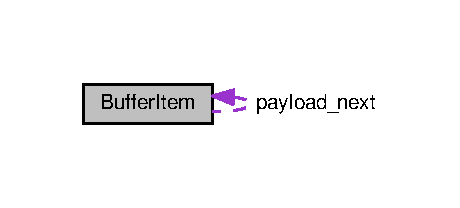
\includegraphics[width=221pt]{structBufferItem__coll__graph}
\end{center}
\end{figure}
\subsection*{Public Attributes}
\begin{DoxyCompactItemize}
\item 
uint8\+\_\+t \hyperlink{structBufferItem_a5c3187c383ceec1825964d5e512273de}{payload\+\_\+size} = 0
\item 
uint8\+\_\+t \hyperlink{structBufferItem_a2e475a18a6671f1f0c4bf3010d7a6e89}{payload\+\_\+destination} = 0
\item 
\hyperlink{structBufferItem}{Buffer\+Item} $\ast$ \hyperlink{structBufferItem_ab20f3ae7cc41c118265557f2c7e2c4f0}{payload\+\_\+next} = 0
\item 
void $\ast$ \hyperlink{structBufferItem_a0ec6d94d7df8c1e9db526fa0200267bb}{payload} = 0
\end{DoxyCompactItemize}


\subsection{Member Data Documentation}
\mbox{\Hypertarget{structBufferItem_a0ec6d94d7df8c1e9db526fa0200267bb}\label{structBufferItem_a0ec6d94d7df8c1e9db526fa0200267bb}} 
\index{Buffer\+Item@{Buffer\+Item}!payload@{payload}}
\index{payload@{payload}!Buffer\+Item@{Buffer\+Item}}
\subsubsection{\texorpdfstring{payload}{payload}}
{\footnotesize\ttfamily void$\ast$ Buffer\+Item\+::payload = 0}

\mbox{\Hypertarget{structBufferItem_a2e475a18a6671f1f0c4bf3010d7a6e89}\label{structBufferItem_a2e475a18a6671f1f0c4bf3010d7a6e89}} 
\index{Buffer\+Item@{Buffer\+Item}!payload\+\_\+destination@{payload\+\_\+destination}}
\index{payload\+\_\+destination@{payload\+\_\+destination}!Buffer\+Item@{Buffer\+Item}}
\subsubsection{\texorpdfstring{payload\+\_\+destination}{payload\_destination}}
{\footnotesize\ttfamily uint8\+\_\+t Buffer\+Item\+::payload\+\_\+destination = 0}

\mbox{\Hypertarget{structBufferItem_ab20f3ae7cc41c118265557f2c7e2c4f0}\label{structBufferItem_ab20f3ae7cc41c118265557f2c7e2c4f0}} 
\index{Buffer\+Item@{Buffer\+Item}!payload\+\_\+next@{payload\+\_\+next}}
\index{payload\+\_\+next@{payload\+\_\+next}!Buffer\+Item@{Buffer\+Item}}
\subsubsection{\texorpdfstring{payload\+\_\+next}{payload\_next}}
{\footnotesize\ttfamily \hyperlink{structBufferItem}{Buffer\+Item}$\ast$ Buffer\+Item\+::payload\+\_\+next = 0}

\mbox{\Hypertarget{structBufferItem_a5c3187c383ceec1825964d5e512273de}\label{structBufferItem_a5c3187c383ceec1825964d5e512273de}} 
\index{Buffer\+Item@{Buffer\+Item}!payload\+\_\+size@{payload\+\_\+size}}
\index{payload\+\_\+size@{payload\+\_\+size}!Buffer\+Item@{Buffer\+Item}}
\subsubsection{\texorpdfstring{payload\+\_\+size}{payload\_size}}
{\footnotesize\ttfamily uint8\+\_\+t Buffer\+Item\+::payload\+\_\+size = 0}



The documentation for this struct was generated from the following file\+:\begin{DoxyCompactItemize}
\item 
\hyperlink{TooNetworking_8h}{Too\+Networking.\+h}\end{DoxyCompactItemize}

\hypertarget{structNoncePayload}{}\section{Nonce\+Payload Struct Reference}
\label{structNoncePayload}\index{Nonce\+Payload@{Nonce\+Payload}}


{\ttfamily \#include $<$Too\+Networking.\+h$>$}

\subsection*{Public Attributes}
\begin{DoxyCompactItemize}
\item 
uint32\+\_\+t \hyperlink{structNoncePayload_ac738ccf9734f52407eef0b48bdf6cb01}{nonce} = 0
\end{DoxyCompactItemize}


\subsection{Detailed Description}
Used to simplify sending nonce replies 

\subsection{Member Data Documentation}
\mbox{\Hypertarget{structNoncePayload_ac738ccf9734f52407eef0b48bdf6cb01}\label{structNoncePayload_ac738ccf9734f52407eef0b48bdf6cb01}} 
\index{Nonce\+Payload@{Nonce\+Payload}!nonce@{nonce}}
\index{nonce@{nonce}!Nonce\+Payload@{Nonce\+Payload}}
\subsubsection{\texorpdfstring{nonce}{nonce}}
{\footnotesize\ttfamily uint32\+\_\+t Nonce\+Payload\+::nonce = 0}



The documentation for this struct was generated from the following file\+:\begin{DoxyCompactItemize}
\item 
\hyperlink{TooNetworking_8h}{Too\+Networking.\+h}\end{DoxyCompactItemize}

\hypertarget{structNonceReceived}{}\section{Nonce\+Received Struct Reference}
\label{structNonceReceived}\index{Nonce\+Received@{Nonce\+Received}}


{\ttfamily \#include $<$Too\+Networking.\+h$>$}



Collaboration diagram for Nonce\+Received\+:
\nopagebreak
\begin{figure}[H]
\begin{center}
\leavevmode
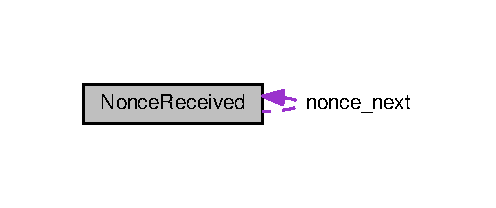
\includegraphics[width=238pt]{structNonceReceived__coll__graph}
\end{center}
\end{figure}
\subsection*{Public Attributes}
\begin{DoxyCompactItemize}
\item 
uint8\+\_\+t \hyperlink{structNonceReceived_aa6f2777bb591400ce057bd1fa9b23fca}{nonce\+\_\+from} = 255
\item 
uint32\+\_\+t \hyperlink{structNonceReceived_adce029bb8f1d7bb73522ed06efca86c0}{nonce\+\_\+time} = 0
\item 
uint32\+\_\+t \hyperlink{structNonceReceived_a39c9b5816fb33fe66f80c8bf98eca7d5}{nonce\+\_\+timestamp} = 0
\item 
\hyperlink{structNonceReceived}{Nonce\+Received} $\ast$ \hyperlink{structNonceReceived_abfc581a902d83cac731aa843feeea5e2}{nonce\+\_\+next} = 0
\end{DoxyCompactItemize}


\subsection{Detailed Description}
Used for storing the nonce and metadata 

\subsection{Member Data Documentation}
\mbox{\Hypertarget{structNonceReceived_aa6f2777bb591400ce057bd1fa9b23fca}\label{structNonceReceived_aa6f2777bb591400ce057bd1fa9b23fca}} 
\index{Nonce\+Received@{Nonce\+Received}!nonce\+\_\+from@{nonce\+\_\+from}}
\index{nonce\+\_\+from@{nonce\+\_\+from}!Nonce\+Received@{Nonce\+Received}}
\subsubsection{\texorpdfstring{nonce\+\_\+from}{nonce\_from}}
{\footnotesize\ttfamily uint8\+\_\+t Nonce\+Received\+::nonce\+\_\+from = 255}

\mbox{\Hypertarget{structNonceReceived_abfc581a902d83cac731aa843feeea5e2}\label{structNonceReceived_abfc581a902d83cac731aa843feeea5e2}} 
\index{Nonce\+Received@{Nonce\+Received}!nonce\+\_\+next@{nonce\+\_\+next}}
\index{nonce\+\_\+next@{nonce\+\_\+next}!Nonce\+Received@{Nonce\+Received}}
\subsubsection{\texorpdfstring{nonce\+\_\+next}{nonce\_next}}
{\footnotesize\ttfamily \hyperlink{structNonceReceived}{Nonce\+Received}$\ast$ Nonce\+Received\+::nonce\+\_\+next = 0}

\mbox{\Hypertarget{structNonceReceived_adce029bb8f1d7bb73522ed06efca86c0}\label{structNonceReceived_adce029bb8f1d7bb73522ed06efca86c0}} 
\index{Nonce\+Received@{Nonce\+Received}!nonce\+\_\+time@{nonce\+\_\+time}}
\index{nonce\+\_\+time@{nonce\+\_\+time}!Nonce\+Received@{Nonce\+Received}}
\subsubsection{\texorpdfstring{nonce\+\_\+time}{nonce\_time}}
{\footnotesize\ttfamily uint32\+\_\+t Nonce\+Received\+::nonce\+\_\+time = 0}

\mbox{\Hypertarget{structNonceReceived_a39c9b5816fb33fe66f80c8bf98eca7d5}\label{structNonceReceived_a39c9b5816fb33fe66f80c8bf98eca7d5}} 
\index{Nonce\+Received@{Nonce\+Received}!nonce\+\_\+timestamp@{nonce\+\_\+timestamp}}
\index{nonce\+\_\+timestamp@{nonce\+\_\+timestamp}!Nonce\+Received@{Nonce\+Received}}
\subsubsection{\texorpdfstring{nonce\+\_\+timestamp}{nonce\_timestamp}}
{\footnotesize\ttfamily uint32\+\_\+t Nonce\+Received\+::nonce\+\_\+timestamp = 0}



The documentation for this struct was generated from the following file\+:\begin{DoxyCompactItemize}
\item 
\hyperlink{TooNetworking_8h}{Too\+Networking.\+h}\end{DoxyCompactItemize}

\hypertarget{structNonceRequested}{}\section{Nonce\+Requested Struct Reference}
\label{structNonceRequested}\index{Nonce\+Requested@{Nonce\+Requested}}


{\ttfamily \#include $<$Too\+Networking\+\_\+data.\+h$>$}



Collaboration diagram for Nonce\+Requested\+:\nopagebreak
\begin{figure}[H]
\begin{center}
\leavevmode
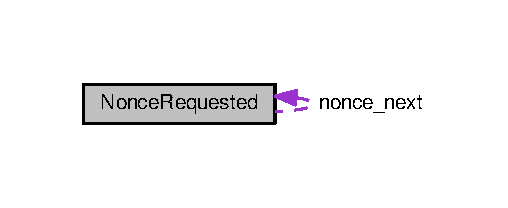
\includegraphics[width=212pt]{structNonceRequested__coll__graph}
\end{center}
\end{figure}
\subsection*{Public Attributes}
\begin{DoxyCompactItemize}
\item 
uint8\+\_\+t \hyperlink{structNonceRequested_a49d5f4e83fa72e51cc37237cc46f3a7e}{nonce\+\_\+from} = 255
\item 
uint32\+\_\+t \hyperlink{structNonceRequested_a9e2f47eec20e01c7cce1acf2d47bbf14}{nonce\+\_\+request\+\_\+first} = 0
\item 
uint32\+\_\+t \hyperlink{structNonceRequested_ae5453d115c1ba4044592921e0127f0c8}{nonce\+\_\+request\+\_\+last} = 0
\item 
\hyperlink{structNonceRequested}{Nonce\+Requested} $\ast$ \hyperlink{structNonceRequested_a2ef35667b6b2cb12f1c845ddc63f16ec}{next} = 0
\end{DoxyCompactItemize}


\subsection{Detailed Description}
Used for storing metadata about nonce requests 

\subsection{Member Data Documentation}
\mbox{\Hypertarget{structNonceRequested_a2ef35667b6b2cb12f1c845ddc63f16ec}\label{structNonceRequested_a2ef35667b6b2cb12f1c845ddc63f16ec}} 
\index{Nonce\+Requested@{Nonce\+Requested}!next@{next}}
\index{next@{next}!Nonce\+Requested@{Nonce\+Requested}}
\subsubsection{\texorpdfstring{next}{next}}
{\footnotesize\ttfamily \hyperlink{structNonceRequested}{Nonce\+Requested}$\ast$ Nonce\+Requested\+::next = 0}

Next in the list \mbox{\Hypertarget{structNonceRequested_a49d5f4e83fa72e51cc37237cc46f3a7e}\label{structNonceRequested_a49d5f4e83fa72e51cc37237cc46f3a7e}} 
\index{Nonce\+Requested@{Nonce\+Requested}!nonce\+\_\+from@{nonce\+\_\+from}}
\index{nonce\+\_\+from@{nonce\+\_\+from}!Nonce\+Requested@{Nonce\+Requested}}
\subsubsection{\texorpdfstring{nonce\+\_\+from}{nonce\_from}}
{\footnotesize\ttfamily uint8\+\_\+t Nonce\+Requested\+::nonce\+\_\+from = 255}

Requested from \mbox{\Hypertarget{structNonceRequested_a9e2f47eec20e01c7cce1acf2d47bbf14}\label{structNonceRequested_a9e2f47eec20e01c7cce1acf2d47bbf14}} 
\index{Nonce\+Requested@{Nonce\+Requested}!nonce\+\_\+request\+\_\+first@{nonce\+\_\+request\+\_\+first}}
\index{nonce\+\_\+request\+\_\+first@{nonce\+\_\+request\+\_\+first}!Nonce\+Requested@{Nonce\+Requested}}
\subsubsection{\texorpdfstring{nonce\+\_\+request\+\_\+first}{nonce\_request\_first}}
{\footnotesize\ttfamily uint32\+\_\+t Nonce\+Requested\+::nonce\+\_\+request\+\_\+first = 0}

First request time \mbox{\Hypertarget{structNonceRequested_ae5453d115c1ba4044592921e0127f0c8}\label{structNonceRequested_ae5453d115c1ba4044592921e0127f0c8}} 
\index{Nonce\+Requested@{Nonce\+Requested}!nonce\+\_\+request\+\_\+last@{nonce\+\_\+request\+\_\+last}}
\index{nonce\+\_\+request\+\_\+last@{nonce\+\_\+request\+\_\+last}!Nonce\+Requested@{Nonce\+Requested}}
\subsubsection{\texorpdfstring{nonce\+\_\+request\+\_\+last}{nonce\_request\_last}}
{\footnotesize\ttfamily uint32\+\_\+t Nonce\+Requested\+::nonce\+\_\+request\+\_\+last = 0}

Last request time 

The documentation for this struct was generated from the following file\+:\begin{DoxyCompactItemize}
\item 
\hyperlink{TooNetworking__data_8h}{Too\+Networking\+\_\+data.\+h}\end{DoxyCompactItemize}

\hypertarget{structNonceSent}{}\section{Nonce\+Sent Struct Reference}
\label{structNonceSent}\index{Nonce\+Sent@{Nonce\+Sent}}


{\ttfamily \#include $<$Too\+Networking.\+h$>$}



Collaboration diagram for Nonce\+Sent\+:\nopagebreak
\begin{figure}[H]
\begin{center}
\leavevmode
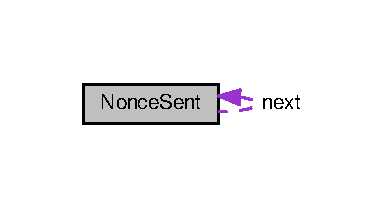
\includegraphics[width=185pt]{structNonceSent__coll__graph}
\end{center}
\end{figure}
\subsection*{Public Attributes}
\begin{DoxyCompactItemize}
\item 
uint8\+\_\+t \hyperlink{structNonceSent_ad5484888a11a0c041610c38b564c5627}{nonce\+\_\+to} = 255
\item 
uint32\+\_\+t \hyperlink{structNonceSent_ae9d167a911c22c9d4490d2fee2093c10}{nonce} = 0
\item 
\hyperlink{structNonceSent}{Nonce\+Sent} $\ast$ \hyperlink{structNonceSent_a1c51c6d93e58ff1d94a0ab691c28fd24}{next} = 0
\end{DoxyCompactItemize}


\subsection{Detailed Description}
Used for storing metadata and the nonce sent to other nodes in the network 

\subsection{Member Data Documentation}
\index{Nonce\+Sent@{Nonce\+Sent}!next@{next}}
\index{next@{next}!Nonce\+Sent@{Nonce\+Sent}}
\subsubsection[{\texorpdfstring{next}{next}}]{\setlength{\rightskip}{0pt plus 5cm}{\bf Nonce\+Sent}$\ast$ Nonce\+Sent\+::next = 0}\hypertarget{structNonceSent_a1c51c6d93e58ff1d94a0ab691c28fd24}{}\label{structNonceSent_a1c51c6d93e58ff1d94a0ab691c28fd24}
Next item in the list \index{Nonce\+Sent@{Nonce\+Sent}!nonce@{nonce}}
\index{nonce@{nonce}!Nonce\+Sent@{Nonce\+Sent}}
\subsubsection[{\texorpdfstring{nonce}{nonce}}]{\setlength{\rightskip}{0pt plus 5cm}uint32\+\_\+t Nonce\+Sent\+::nonce = 0}\hypertarget{structNonceSent_ae9d167a911c22c9d4490d2fee2093c10}{}\label{structNonceSent_ae9d167a911c22c9d4490d2fee2093c10}
Nonce itself \index{Nonce\+Sent@{Nonce\+Sent}!nonce\+\_\+to@{nonce\+\_\+to}}
\index{nonce\+\_\+to@{nonce\+\_\+to}!Nonce\+Sent@{Nonce\+Sent}}
\subsubsection[{\texorpdfstring{nonce\+\_\+to}{nonce_to}}]{\setlength{\rightskip}{0pt plus 5cm}uint8\+\_\+t Nonce\+Sent\+::nonce\+\_\+to = 255}\hypertarget{structNonceSent_ad5484888a11a0c041610c38b564c5627}{}\label{structNonceSent_ad5484888a11a0c041610c38b564c5627}
Destination 

The documentation for this struct was generated from the following file\+:\begin{DoxyCompactItemize}
\item 
\hyperlink{TooNetworking_8h}{Too\+Networking.\+h}\end{DoxyCompactItemize}

\hypertarget{structPayload__Metadata__Received}{}\section{Payload\+\_\+\+Metadata\+\_\+\+Received Struct Reference}
\label{structPayload__Metadata__Received}\index{Payload\+\_\+\+Metadata\+\_\+\+Received@{Payload\+\_\+\+Metadata\+\_\+\+Received}}


{\ttfamily \#include $<$Too\+Networking.\+h$>$}

\subsection*{Public Attributes}
\begin{DoxyCompactItemize}
\item 
uint8\+\_\+t \hyperlink{structPayload__Metadata__Received_a4dcd8b5b8c5a4565f1bac2fc4212bf71}{payload\+\_\+size}
\item 
uint8\+\_\+t \hyperlink{structPayload__Metadata__Received_a0105d708c3cc157a95c3cf4068e290de}{payload\+\_\+type}
\end{DoxyCompactItemize}


\subsection{Detailed Description}
Used for reading the required payload size to properly deal with the payloads

This is actually inside the sent and received payloads unlike the rest of the data in \hyperlink{structBufferItem}{Buffer\+Item} or Buffer\+Item\+\_\+\+Signed 

\subsection{Member Data Documentation}
\index{Payload\+\_\+\+Metadata\+\_\+\+Received@{Payload\+\_\+\+Metadata\+\_\+\+Received}!payload\+\_\+size@{payload\+\_\+size}}
\index{payload\+\_\+size@{payload\+\_\+size}!Payload\+\_\+\+Metadata\+\_\+\+Received@{Payload\+\_\+\+Metadata\+\_\+\+Received}}
\subsubsection[{\texorpdfstring{payload\+\_\+size}{payload_size}}]{\setlength{\rightskip}{0pt plus 5cm}uint8\+\_\+t Payload\+\_\+\+Metadata\+\_\+\+Received\+::payload\+\_\+size}\hypertarget{structPayload__Metadata__Received_a4dcd8b5b8c5a4565f1bac2fc4212bf71}{}\label{structPayload__Metadata__Received_a4dcd8b5b8c5a4565f1bac2fc4212bf71}
Received payload size \index{Payload\+\_\+\+Metadata\+\_\+\+Received@{Payload\+\_\+\+Metadata\+\_\+\+Received}!payload\+\_\+type@{payload\+\_\+type}}
\index{payload\+\_\+type@{payload\+\_\+type}!Payload\+\_\+\+Metadata\+\_\+\+Received@{Payload\+\_\+\+Metadata\+\_\+\+Received}}
\subsubsection[{\texorpdfstring{payload\+\_\+type}{payload_type}}]{\setlength{\rightskip}{0pt plus 5cm}uint8\+\_\+t Payload\+\_\+\+Metadata\+\_\+\+Received\+::payload\+\_\+type}\hypertarget{structPayload__Metadata__Received_a0105d708c3cc157a95c3cf4068e290de}{}\label{structPayload__Metadata__Received_a0105d708c3cc157a95c3cf4068e290de}
Received payload type, to deal with messages signed, encrypted or both 

The documentation for this struct was generated from the following file\+:\begin{DoxyCompactItemize}
\item 
\hyperlink{TooNetworking_8h}{Too\+Networking.\+h}\end{DoxyCompactItemize}

\hypertarget{structPayload__MetadataSigned__Received}{}\section{Payload\+\_\+\+Metadata\+Signed\+\_\+\+Received Struct Reference}
\label{structPayload__MetadataSigned__Received}\index{Payload\+\_\+\+Metadata\+Signed\+\_\+\+Received@{Payload\+\_\+\+Metadata\+Signed\+\_\+\+Received}}


{\ttfamily \#include $<$Too\+Networking.\+h$>$}

\subsection*{Public Attributes}
\begin{DoxyCompactItemize}
\item 
uint8\+\_\+t \hyperlink{structPayload__MetadataSigned__Received_a3d2d5a1f14940bbc0435dc1fec8fb238}{payload\+\_\+size}
\item 
uint8\+\_\+t \hyperlink{structPayload__MetadataSigned__Received_aad832d1e40428c42d4cac30012eacc02}{payload\+\_\+type}
\item 
uint8\+\_\+t \hyperlink{structPayload__MetadataSigned__Received_a6c37ad37ff363c7480fa99836fbdc0c5}{payload\+\_\+hash} \mbox{[}32\mbox{]}
\end{DoxyCompactItemize}


\subsection{Detailed Description}
Used for reading the required hash, payload type and size to properly deal with received signed payloads 

\subsection{Member Data Documentation}
\index{Payload\+\_\+\+Metadata\+Signed\+\_\+\+Received@{Payload\+\_\+\+Metadata\+Signed\+\_\+\+Received}!payload\+\_\+hash@{payload\+\_\+hash}}
\index{payload\+\_\+hash@{payload\+\_\+hash}!Payload\+\_\+\+Metadata\+Signed\+\_\+\+Received@{Payload\+\_\+\+Metadata\+Signed\+\_\+\+Received}}
\subsubsection[{\texorpdfstring{payload\+\_\+hash}{payload_hash}}]{\setlength{\rightskip}{0pt plus 5cm}uint8\+\_\+t Payload\+\_\+\+Metadata\+Signed\+\_\+\+Received\+::payload\+\_\+hash\mbox{[}32\mbox{]}}\hypertarget{structPayload__MetadataSigned__Received_a6c37ad37ff363c7480fa99836fbdc0c5}{}\label{structPayload__MetadataSigned__Received_a6c37ad37ff363c7480fa99836fbdc0c5}
Payload hash generated by the source \index{Payload\+\_\+\+Metadata\+Signed\+\_\+\+Received@{Payload\+\_\+\+Metadata\+Signed\+\_\+\+Received}!payload\+\_\+size@{payload\+\_\+size}}
\index{payload\+\_\+size@{payload\+\_\+size}!Payload\+\_\+\+Metadata\+Signed\+\_\+\+Received@{Payload\+\_\+\+Metadata\+Signed\+\_\+\+Received}}
\subsubsection[{\texorpdfstring{payload\+\_\+size}{payload_size}}]{\setlength{\rightskip}{0pt plus 5cm}uint8\+\_\+t Payload\+\_\+\+Metadata\+Signed\+\_\+\+Received\+::payload\+\_\+size}\hypertarget{structPayload__MetadataSigned__Received_a3d2d5a1f14940bbc0435dc1fec8fb238}{}\label{structPayload__MetadataSigned__Received_a3d2d5a1f14940bbc0435dc1fec8fb238}
Received payload size \index{Payload\+\_\+\+Metadata\+Signed\+\_\+\+Received@{Payload\+\_\+\+Metadata\+Signed\+\_\+\+Received}!payload\+\_\+type@{payload\+\_\+type}}
\index{payload\+\_\+type@{payload\+\_\+type}!Payload\+\_\+\+Metadata\+Signed\+\_\+\+Received@{Payload\+\_\+\+Metadata\+Signed\+\_\+\+Received}}
\subsubsection[{\texorpdfstring{payload\+\_\+type}{payload_type}}]{\setlength{\rightskip}{0pt plus 5cm}uint8\+\_\+t Payload\+\_\+\+Metadata\+Signed\+\_\+\+Received\+::payload\+\_\+type}\hypertarget{structPayload__MetadataSigned__Received_aad832d1e40428c42d4cac30012eacc02}{}\label{structPayload__MetadataSigned__Received_aad832d1e40428c42d4cac30012eacc02}
Received payload type, to deal with messages signed, encrypted or both 

The documentation for this struct was generated from the following file\+:\begin{DoxyCompactItemize}
\item 
\hyperlink{TooNetworking_8h}{Too\+Networking.\+h}\end{DoxyCompactItemize}

\chapter{File Documentation}
\hypertarget{CONTRIBUTING_8md}{}\section{C\+O\+N\+T\+R\+I\+B\+U\+T\+I\+N\+G.\+md File Reference}
\label{CONTRIBUTING_8md}\index{C\+O\+N\+T\+R\+I\+B\+U\+T\+I\+N\+G.\+md@{C\+O\+N\+T\+R\+I\+B\+U\+T\+I\+N\+G.\+md}}

\hypertarget{hmacs_8c}{}\section{hmacs.\+c File Reference}
\label{hmacs_8c}\index{hmacs.\+c@{hmacs.\+c}}
\subsection*{Variables}
\begin{DoxyCompactItemize}
\item 
static const uint8\+\_\+t hmacs \mbox{[}2\mbox{]}\mbox{[}20\mbox{]} \hyperlink{hmacs_8c_ac02263bf6ea4f953104ce51ff72b2f75}{P\+R\+O\+G\+M\+EM}
\end{DoxyCompactItemize}


\subsection{Detailed Description}
This file contains the secret H\+M\+AC keys used if signing is enabled 

\subsection{Variable Documentation}
\mbox{\Hypertarget{hmacs_8c_ac02263bf6ea4f953104ce51ff72b2f75}\label{hmacs_8c_ac02263bf6ea4f953104ce51ff72b2f75}} 
\index{hmacs.\+c@{hmacs.\+c}!P\+R\+O\+G\+M\+EM@{P\+R\+O\+G\+M\+EM}}
\index{P\+R\+O\+G\+M\+EM@{P\+R\+O\+G\+M\+EM}!hmacs.\+c@{hmacs.\+c}}
\subsubsection{\texorpdfstring{P\+R\+O\+G\+M\+EM}{PROGMEM}}
{\footnotesize\ttfamily const uint8\+\_\+t hmacs \mbox{[}2\mbox{]}\mbox{[}20\mbox{]} P\+R\+O\+G\+M\+EM\hspace{0.3cm}{\ttfamily [static]}}

{\bfseries Initial value\+:}
\begin{DoxyCode}
= \{
  \{0, 0, 0, 0, 0, 0, 0, 0, 0, 0, 0, 0, 0, 0, 0, 0, 0, 0, 0, 0\},
  \{255, 255, 255, 255, 255, 255, 255, 255, 255, 255, 255, 255, 255, 255, 255, 255, 255, 255, 255, 255\},
\}
\end{DoxyCode}

\hypertarget{modules_2TooNetworking_2README_8md}{}\section{R\+E\+A\+D\+M\+E.\+md File Reference}
\label{modules_2TooNetworking_2README_8md}\index{R\+E\+A\+D\+M\+E.\+md@{R\+E\+A\+D\+M\+E.\+md}}

\hypertarget{modules_2TooSigning_2README_8md}{}\section{R\+E\+A\+D\+M\+E.\+md File Reference}
\label{modules_2TooSigning_2README_8md}\index{R\+E\+A\+D\+M\+E.\+md@{R\+E\+A\+D\+M\+E.\+md}}

\hypertarget{README_8md}{}\section{R\+E\+A\+D\+M\+E.\+md File Reference}
\label{README_8md}\index{R\+E\+A\+D\+M\+E.\+md@{R\+E\+A\+D\+M\+E.\+md}}

\hypertarget{TooAutomation_8h}{}\section{Too\+Automation.\+h File Reference}
\label{TooAutomation_8h}\index{Too\+Automation.\+h@{Too\+Automation.\+h}}

\hypertarget{TooInput_8h}{}\section{Too\+Input.\+h File Reference}
\label{TooInput_8h}\index{Too\+Input.\+h@{Too\+Input.\+h}}


\subsection{Detailed Description}
This file implements the necessary functionality that allow nodes to collect data 
\hypertarget{TooNetworking_8h}{}\section{Too\+Networking.\+h File Reference}
\label{TooNetworking_8h}\index{Too\+Networking.\+h@{Too\+Networking.\+h}}
\subsection*{Classes}
\begin{DoxyCompactItemize}
\item 
struct \hyperlink{structBufferItem}{Buffer\+Item}
\item 
struct \hyperlink{structPayload__Metadata}{Payload\+\_\+\+Metadata}
\item 
struct \hyperlink{structPayload__MetadataSigned}{Payload\+\_\+\+Metadata\+Signed}
\item 
struct \hyperlink{structBufferItem__Signed}{Buffer\+Item\+\_\+\+Signed}
\item 
struct \hyperlink{structNonceSent}{Nonce\+Sent}
\item 
struct \hyperlink{structNonceReceived}{Nonce\+Received}
\item 
struct \hyperlink{structNoncePayload}{Nonce\+Payload}
\item 
struct \hyperlink{structNonceRequested}{Nonce\+Requested}
\end{DoxyCompactItemize}
\subsection*{Functions}
\begin{DoxyCompactItemize}
\item 
R\+F24 \hyperlink{TooNetworking_8h_a173f695381b08642c89a68cdcd76a5d4}{radio} (T\+O\+O\+\_\+\+R\+F24\+\_\+\+CE, T\+O\+O\+\_\+\+R\+F24\+\_\+\+CS)
\item 
R\+F24\+Network \hyperlink{TooNetworking_8h_aa7924d94ea32c8d33a81ff41f8678320}{network} (\hyperlink{TooNetworking_8h_a173f695381b08642c89a68cdcd76a5d4}{radio})
\item 
R\+F24\+Mesh \hyperlink{TooNetworking_8h_abdda8f09b9d475ed2c23a2376e2e0151}{mesh} (\hyperlink{TooNetworking_8h_a173f695381b08642c89a68cdcd76a5d4}{radio}, \hyperlink{TooNetworking_8h_aa7924d94ea32c8d33a81ff41f8678320}{network})
\item 
bool \hyperlink{TooNetworking_8h_aec97902cf0d3ec10fd86927f3d1df0c6}{Too\+Networking\+\_\+connection\+\_\+begin} (uint8\+\_\+t passed\+\_\+node\+\_\+id)
\item 
bool \hyperlink{TooNetworking_8h_a723608b997230cc461d06454b2cdb8c3}{Too\+Networking\+\_\+send} (uint8\+\_\+t for\+\_\+node, void $\ast$payload, uint8\+\_\+t size, uint8\+\_\+t type)
\item 
bool \hyperlink{TooNetworking_8h_a9209f3e1a2fdf0b3b88d49105b8fc359}{Too\+Networking\+\_\+send\+\_\+signed} (uint8\+\_\+t for\+\_\+node, void $\ast$payload, uint8\+\_\+t size)
\item 
bool \hyperlink{TooNetworking_8h_a9f893c3218491ee86282fdcd9f376500}{Too\+Networking\+\_\+send\+\_\+signed\+\_\+} (uint8\+\_\+t for\+\_\+node, void $\ast$payload, uint8\+\_\+t size, uint32\+\_\+t nonce)
\item 
bool \hyperlink{TooNetworking_8h_a86fb32acfc42a498be62a3236c778454}{Too\+Networking\+\_\+send\+\_\+encrypted} (uint8\+\_\+t for\+\_\+node, void $\ast$payload, uint8\+\_\+t size)
\item 
bool \hyperlink{TooNetworking_8h_a5861e5d6df60aa6701af1b9ec7e942a8}{Too\+Networking\+\_\+send\+\_\+signed\+\_\+encrypted} (uint8\+\_\+t for\+\_\+node, void $\ast$payload, uint8\+\_\+t size)
\item 
bool \hyperlink{TooNetworking_8h_a8b2b7fde063d7268ae7deabffeba6152}{Too\+Networking\+\_\+peek} (R\+F24\+Network\+Header \&header, void $\ast$message, uint16\+\_\+t maxlen)
\item 
bool \hyperlink{TooNetworking_8h_a9cd17becc197be8de7befa25116c3a67}{Too\+Networking\+\_\+read} (R\+F24\+Network\+Header \&header, void $\ast$message, uint16\+\_\+t maxlen)
\item 
bool \hyperlink{TooNetworking_8h_ac352268e177fa2ddf91c8afa5cd04bbf}{Too\+Networking\+\_\+connection\+\_\+available} ()
\item 
bool \hyperlink{TooNetworking_8h_a48504aef69d9ac92e34269a64f7b518b}{Too\+Networking\+\_\+connection\+\_\+check} ()
\item 
bool \hyperlink{TooNetworking_8h_aefc5dad88b637efb11a3a7b2f76a19b9}{Too\+Networking\+\_\+connection\+\_\+fix} ()
\item 
bool \hyperlink{TooNetworking_8h_a7382ba1aed5405c3adc02011ea6c45dd}{Too\+Networking\+\_\+connection\+\_\+maintenance} ()
\item 
void \hyperlink{group__SIMPLE__BUFFER_ga3c91b7ab2f6500c287ecc7ab4a018ef6}{Too\+Networking\+\_\+bufferlist\+\_\+remove} (\hyperlink{structBufferItem}{Buffer\+Item} $\ast$previous, \hyperlink{structBufferItem}{Buffer\+Item} $\ast$current)
\item 
bool \hyperlink{group__SIMPLE__BUFFER_gaa8a4e879d4d71fed2a8940cf93b75ae4}{Too\+Networking\+\_\+bufferlist\+\_\+initialize} ()
\item 
\hyperlink{structBufferItem}{Buffer\+Item} $\ast$ \hyperlink{group__SIMPLE__BUFFER_ga0dd5e9de81eea99b99669a607c9b4028}{Too\+Networking\+\_\+bufferlist\+\_\+find\+\_\+for\+\_\+id} (uint8\+\_\+t node\+ID)
\item 
bool \hyperlink{group__SIMPLE__BUFFER_gae72372a8084e8486f1306240a9af6474}{Too\+Networking\+\_\+bufferlist\+\_\+send} (\hyperlink{structBufferItem}{Buffer\+Item} $\ast$item, \hyperlink{structNonceReceived}{Nonce\+Received} $\ast$nonce, \hyperlink{structBufferItem}{Buffer\+Item} $\ast$previousitem)
\item 
bool \hyperlink{group__SIMPLE__BUFFER_ga1fca7e85a8a2f91a1b20a8bb23b4e893}{Too\+Networking\+\_\+bufferlist\+\_\+add} (uint8\+\_\+t payload\+\_\+destination, void $\ast$payload, uint8\+\_\+t size)
\item 
void \hyperlink{group__SIMPLE__BUFFER_gab58e06e0eb6f2f8ecbebeaf3c173fb22}{Too\+Networking\+\_\+bufferlist\+\_\+send\+\_\+all} ()
\item 
void \hyperlink{group__SIMPLE__BUFFER_ga2b5485b317146ce7c14bbad26172d796}{Too\+Networking\+\_\+bufferlist\+\_\+print} ()
\item 
bool \hyperlink{TooNetworking_8h_aa9ec1ce0a58a96d0452a5ec51bb0bfca}{Too\+Neteorking\+\_\+connection\+\_\+fix} ()
\item 
bool \hyperlink{TooNetworking_8h_a2676204dee95da1ef337de95eb0e9bcb}{Too\+Networking\+\_\+begin} (uint8\+\_\+t passed\+\_\+node\+\_\+id)
\end{DoxyCompactItemize}
\subsection*{Variables}
\begin{DoxyCompactItemize}
\item 
uint8\+\_\+t \hyperlink{TooNetworking_8h_a4277db94d928ddb590684b5bf9174f73}{current\+\_\+node\+\_\+\+ID}
\item 
Sha256\+Class \hyperlink{TooNetworking_8h_a2cde2cc921aef77784b8d5b3129b5803}{Sha256}
\item 
\hyperlink{structNonceSent}{Nonce\+Sent} $\ast$ \hyperlink{TooNetworking_8h_ae75ffa3e0a98255f366188a6223156bc}{nonce\+\_\+sent\+\_\+start} = 0
\item 
\hyperlink{structNonceReceived}{Nonce\+Received} $\ast$ \hyperlink{TooNetworking_8h_ad145f92b978c39b1728ffd91e896277a}{nonce\+\_\+received\+\_\+start} = 0
\item 
\hyperlink{structNonceRequested}{Nonce\+Requested} $\ast$ \hyperlink{TooNetworking_8h_aac43930ae93d50eea7e1ae8aee603524}{nonce\+\_\+requested\+\_\+first} = 0
\item 
\hyperlink{structBufferItem}{Buffer\+Item} $\ast$ \hyperlink{TooNetworking_8h_a7c24840cd9eb766eb04c1db0d2363cd5}{buffer\+\_\+first} = 0
\end{DoxyCompactItemize}


\subsection{Detailed Description}
This file implements the necessary functionality that allow nodes in the network to communicate 

\subsection{Function Documentation}
\mbox{\Hypertarget{TooNetworking_8h_abdda8f09b9d475ed2c23a2376e2e0151}\label{TooNetworking_8h_abdda8f09b9d475ed2c23a2376e2e0151}} 
\index{Too\+Networking.\+h@{Too\+Networking.\+h}!mesh@{mesh}}
\index{mesh@{mesh}!Too\+Networking.\+h@{Too\+Networking.\+h}}
\subsubsection{\texorpdfstring{mesh()}{mesh()}}
{\footnotesize\ttfamily R\+F24\+Mesh mesh (\begin{DoxyParamCaption}\item[{\hyperlink{TooNetworking_8h_a173f695381b08642c89a68cdcd76a5d4}{radio}}]{,  }\item[{\hyperlink{TooNetworking_8h_aa7924d94ea32c8d33a81ff41f8678320}{network}}]{ }\end{DoxyParamCaption})}

\mbox{\Hypertarget{TooNetworking_8h_aa7924d94ea32c8d33a81ff41f8678320}\label{TooNetworking_8h_aa7924d94ea32c8d33a81ff41f8678320}} 
\index{Too\+Networking.\+h@{Too\+Networking.\+h}!network@{network}}
\index{network@{network}!Too\+Networking.\+h@{Too\+Networking.\+h}}
\subsubsection{\texorpdfstring{network()}{network()}}
{\footnotesize\ttfamily R\+F24\+Network network (\begin{DoxyParamCaption}\item[{\hyperlink{TooNetworking_8h_a173f695381b08642c89a68cdcd76a5d4}{radio}}]{ }\end{DoxyParamCaption})}

\mbox{\Hypertarget{TooNetworking_8h_a173f695381b08642c89a68cdcd76a5d4}\label{TooNetworking_8h_a173f695381b08642c89a68cdcd76a5d4}} 
\index{Too\+Networking.\+h@{Too\+Networking.\+h}!radio@{radio}}
\index{radio@{radio}!Too\+Networking.\+h@{Too\+Networking.\+h}}
\subsubsection{\texorpdfstring{radio()}{radio()}}
{\footnotesize\ttfamily R\+F24 radio (\begin{DoxyParamCaption}\item[{T\+O\+O\+\_\+\+R\+F24\+\_\+\+CE}]{,  }\item[{T\+O\+O\+\_\+\+R\+F24\+\_\+\+CS}]{ }\end{DoxyParamCaption})}

\mbox{\Hypertarget{TooNetworking_8h_aa9ec1ce0a58a96d0452a5ec51bb0bfca}\label{TooNetworking_8h_aa9ec1ce0a58a96d0452a5ec51bb0bfca}} 
\index{Too\+Networking.\+h@{Too\+Networking.\+h}!Too\+Neteorking\+\_\+connection\+\_\+fix@{Too\+Neteorking\+\_\+connection\+\_\+fix}}
\index{Too\+Neteorking\+\_\+connection\+\_\+fix@{Too\+Neteorking\+\_\+connection\+\_\+fix}!Too\+Networking.\+h@{Too\+Networking.\+h}}
\subsubsection{\texorpdfstring{Too\+Neteorking\+\_\+connection\+\_\+fix()}{TooNeteorking\_connection\_fix()}}
{\footnotesize\ttfamily bool Too\+Neteorking\+\_\+connection\+\_\+fix (\begin{DoxyParamCaption}{ }\end{DoxyParamCaption})}

Tries to reestablish connection to the network

\begin{DoxyReturn}{Returns}
True if successful, false otherwise 
\end{DoxyReturn}
\mbox{\Hypertarget{TooNetworking_8h_a2676204dee95da1ef337de95eb0e9bcb}\label{TooNetworking_8h_a2676204dee95da1ef337de95eb0e9bcb}} 
\index{Too\+Networking.\+h@{Too\+Networking.\+h}!Too\+Networking\+\_\+begin@{Too\+Networking\+\_\+begin}}
\index{Too\+Networking\+\_\+begin@{Too\+Networking\+\_\+begin}!Too\+Networking.\+h@{Too\+Networking.\+h}}
\subsubsection{\texorpdfstring{Too\+Networking\+\_\+begin()}{TooNetworking\_begin()}}
{\footnotesize\ttfamily bool Too\+Networking\+\_\+begin (\begin{DoxyParamCaption}\item[{uint8\+\_\+t}]{passed\+\_\+node\+\_\+id }\end{DoxyParamCaption})}

Automatically set up the networking Every radio should provide \hyperlink{TooNetworking_8h_aec97902cf0d3ec10fd86927f3d1df0c6}{Too\+Networking\+\_\+connection\+\_\+begin(uint8\+\_\+t node\+I\+D)} for easy initialization of the network


\begin{DoxyParams}{Parameters}
{\em passed\+\_\+node\+\_\+id} & Current node\textquotesingle{}s ID. \\
\hline
\end{DoxyParams}
\begin{DoxyReturn}{Returns}
true if successful, false otherwise 
\end{DoxyReturn}
\mbox{\Hypertarget{TooNetworking_8h_ac352268e177fa2ddf91c8afa5cd04bbf}\label{TooNetworking_8h_ac352268e177fa2ddf91c8afa5cd04bbf}} 
\index{Too\+Networking.\+h@{Too\+Networking.\+h}!Too\+Networking\+\_\+connection\+\_\+available@{Too\+Networking\+\_\+connection\+\_\+available}}
\index{Too\+Networking\+\_\+connection\+\_\+available@{Too\+Networking\+\_\+connection\+\_\+available}!Too\+Networking.\+h@{Too\+Networking.\+h}}
\subsubsection{\texorpdfstring{Too\+Networking\+\_\+connection\+\_\+available()}{TooNetworking\_connection\_available()}}
{\footnotesize\ttfamily bool Too\+Networking\+\_\+connection\+\_\+available (\begin{DoxyParamCaption}{ }\end{DoxyParamCaption})}

Checks if there\textquotesingle{}s something ready to be processed

\begin{DoxyReturn}{Returns}
True if successful, false otherwise 
\end{DoxyReturn}
\mbox{\Hypertarget{TooNetworking_8h_aec97902cf0d3ec10fd86927f3d1df0c6}\label{TooNetworking_8h_aec97902cf0d3ec10fd86927f3d1df0c6}} 
\index{Too\+Networking.\+h@{Too\+Networking.\+h}!Too\+Networking\+\_\+connection\+\_\+begin@{Too\+Networking\+\_\+connection\+\_\+begin}}
\index{Too\+Networking\+\_\+connection\+\_\+begin@{Too\+Networking\+\_\+connection\+\_\+begin}!Too\+Networking.\+h@{Too\+Networking.\+h}}
\subsubsection{\texorpdfstring{Too\+Networking\+\_\+connection\+\_\+begin()}{TooNetworking\_connection\_begin()}}
{\footnotesize\ttfamily bool Too\+Networking\+\_\+connection\+\_\+begin (\begin{DoxyParamCaption}\item[{uint8\+\_\+t}]{passed\+\_\+node\+\_\+id }\end{DoxyParamCaption})}

Automatically set up the networking, implementation depends on the radio


\begin{DoxyParams}{Parameters}
{\em passed\+\_\+node\+\_\+id} & Current node\textquotesingle{}s ID. \\
\hline
\end{DoxyParams}
\begin{DoxyReturn}{Returns}
true if successful, false otherwise 
\end{DoxyReturn}
\mbox{\Hypertarget{TooNetworking_8h_a48504aef69d9ac92e34269a64f7b518b}\label{TooNetworking_8h_a48504aef69d9ac92e34269a64f7b518b}} 
\index{Too\+Networking.\+h@{Too\+Networking.\+h}!Too\+Networking\+\_\+connection\+\_\+check@{Too\+Networking\+\_\+connection\+\_\+check}}
\index{Too\+Networking\+\_\+connection\+\_\+check@{Too\+Networking\+\_\+connection\+\_\+check}!Too\+Networking.\+h@{Too\+Networking.\+h}}
\subsubsection{\texorpdfstring{Too\+Networking\+\_\+connection\+\_\+check()}{TooNetworking\_connection\_check()}}
{\footnotesize\ttfamily bool Too\+Networking\+\_\+connection\+\_\+check (\begin{DoxyParamCaption}{ }\end{DoxyParamCaption})}

Checks if the master node is reachable

\begin{DoxyReturn}{Returns}
true if successful, false otherwise 
\end{DoxyReturn}
\mbox{\Hypertarget{TooNetworking_8h_aefc5dad88b637efb11a3a7b2f76a19b9}\label{TooNetworking_8h_aefc5dad88b637efb11a3a7b2f76a19b9}} 
\index{Too\+Networking.\+h@{Too\+Networking.\+h}!Too\+Networking\+\_\+connection\+\_\+fix@{Too\+Networking\+\_\+connection\+\_\+fix}}
\index{Too\+Networking\+\_\+connection\+\_\+fix@{Too\+Networking\+\_\+connection\+\_\+fix}!Too\+Networking.\+h@{Too\+Networking.\+h}}
\subsubsection{\texorpdfstring{Too\+Networking\+\_\+connection\+\_\+fix()}{TooNetworking\_connection\_fix()}}
{\footnotesize\ttfamily bool Too\+Networking\+\_\+connection\+\_\+fix (\begin{DoxyParamCaption}{ }\end{DoxyParamCaption})}

Tries to reestablish connection to the network

\begin{DoxyReturn}{Returns}
True if successful, false otherwise 
\end{DoxyReturn}
\mbox{\Hypertarget{TooNetworking_8h_a7382ba1aed5405c3adc02011ea6c45dd}\label{TooNetworking_8h_a7382ba1aed5405c3adc02011ea6c45dd}} 
\index{Too\+Networking.\+h@{Too\+Networking.\+h}!Too\+Networking\+\_\+connection\+\_\+maintenance@{Too\+Networking\+\_\+connection\+\_\+maintenance}}
\index{Too\+Networking\+\_\+connection\+\_\+maintenance@{Too\+Networking\+\_\+connection\+\_\+maintenance}!Too\+Networking.\+h@{Too\+Networking.\+h}}
\subsubsection{\texorpdfstring{Too\+Networking\+\_\+connection\+\_\+maintenance()}{TooNetworking\_connection\_maintenance()}}
{\footnotesize\ttfamily bool Too\+Networking\+\_\+connection\+\_\+maintenance (\begin{DoxyParamCaption}{ }\end{DoxyParamCaption})}

Does the necessary maintenance and D\+H\+CP(-\/like) actions on the network

\begin{DoxyReturn}{Returns}
True if successful, false otherwise
\end{DoxyReturn}
Does the necessary maintenance on the network

\begin{DoxyReturn}{Returns}
True if successful, false otherwise 
\end{DoxyReturn}
\mbox{\Hypertarget{TooNetworking_8h_a8b2b7fde063d7268ae7deabffeba6152}\label{TooNetworking_8h_a8b2b7fde063d7268ae7deabffeba6152}} 
\index{Too\+Networking.\+h@{Too\+Networking.\+h}!Too\+Networking\+\_\+peek@{Too\+Networking\+\_\+peek}}
\index{Too\+Networking\+\_\+peek@{Too\+Networking\+\_\+peek}!Too\+Networking.\+h@{Too\+Networking.\+h}}
\subsubsection{\texorpdfstring{Too\+Networking\+\_\+peek()}{TooNetworking\_peek()}}
{\footnotesize\ttfamily bool Too\+Networking\+\_\+peek (\begin{DoxyParamCaption}\item[{R\+F24\+Network\+Header \&}]{header,  }\item[{void $\ast$}]{message,  }\item[{uint16\+\_\+t}]{maxlen }\end{DoxyParamCaption})}

Allows reading a message from buffer and it\textquotesingle{}s N\+OT cleared after being read


\begin{DoxyParams}{Parameters}
{\em } & \\
\hline
\end{DoxyParams}
\mbox{\Hypertarget{TooNetworking_8h_a9cd17becc197be8de7befa25116c3a67}\label{TooNetworking_8h_a9cd17becc197be8de7befa25116c3a67}} 
\index{Too\+Networking.\+h@{Too\+Networking.\+h}!Too\+Networking\+\_\+read@{Too\+Networking\+\_\+read}}
\index{Too\+Networking\+\_\+read@{Too\+Networking\+\_\+read}!Too\+Networking.\+h@{Too\+Networking.\+h}}
\subsubsection{\texorpdfstring{Too\+Networking\+\_\+read()}{TooNetworking\_read()}}
{\footnotesize\ttfamily bool Too\+Networking\+\_\+read (\begin{DoxyParamCaption}\item[{R\+F24\+Network\+Header \&}]{header,  }\item[{void $\ast$}]{message,  }\item[{uint16\+\_\+t}]{maxlen }\end{DoxyParamCaption})}

Allows reading a message from buffer and it\textquotesingle{}s cleared after being read


\begin{DoxyParams}{Parameters}
{\em } & \\
\hline
\end{DoxyParams}
\mbox{\Hypertarget{TooNetworking_8h_a723608b997230cc461d06454b2cdb8c3}\label{TooNetworking_8h_a723608b997230cc461d06454b2cdb8c3}} 
\index{Too\+Networking.\+h@{Too\+Networking.\+h}!Too\+Networking\+\_\+send@{Too\+Networking\+\_\+send}}
\index{Too\+Networking\+\_\+send@{Too\+Networking\+\_\+send}!Too\+Networking.\+h@{Too\+Networking.\+h}}
\subsubsection{\texorpdfstring{Too\+Networking\+\_\+send()}{TooNetworking\_send()}}
{\footnotesize\ttfamily bool Too\+Networking\+\_\+send (\begin{DoxyParamCaption}\item[{uint8\+\_\+t}]{for\+\_\+node,  }\item[{void $\ast$}]{payload,  }\item[{uint8\+\_\+t}]{size,  }\item[{uint8\+\_\+t}]{type }\end{DoxyParamCaption})}

Allows sending a encrypted message


\begin{DoxyParams}{Parameters}
{\em } & \\
\hline
\end{DoxyParams}
\mbox{\Hypertarget{TooNetworking_8h_a86fb32acfc42a498be62a3236c778454}\label{TooNetworking_8h_a86fb32acfc42a498be62a3236c778454}} 
\index{Too\+Networking.\+h@{Too\+Networking.\+h}!Too\+Networking\+\_\+send\+\_\+encrypted@{Too\+Networking\+\_\+send\+\_\+encrypted}}
\index{Too\+Networking\+\_\+send\+\_\+encrypted@{Too\+Networking\+\_\+send\+\_\+encrypted}!Too\+Networking.\+h@{Too\+Networking.\+h}}
\subsubsection{\texorpdfstring{Too\+Networking\+\_\+send\+\_\+encrypted()}{TooNetworking\_send\_encrypted()}}
{\footnotesize\ttfamily bool Too\+Networking\+\_\+send\+\_\+encrypted (\begin{DoxyParamCaption}\item[{uint8\+\_\+t}]{for\+\_\+node,  }\item[{void $\ast$}]{payload,  }\item[{uint8\+\_\+t}]{size }\end{DoxyParamCaption})}

Allows sending an encrypted message


\begin{DoxyParams}{Parameters}
{\em } & \\
\hline
\end{DoxyParams}
\mbox{\Hypertarget{TooNetworking_8h_a9209f3e1a2fdf0b3b88d49105b8fc359}\label{TooNetworking_8h_a9209f3e1a2fdf0b3b88d49105b8fc359}} 
\index{Too\+Networking.\+h@{Too\+Networking.\+h}!Too\+Networking\+\_\+send\+\_\+signed@{Too\+Networking\+\_\+send\+\_\+signed}}
\index{Too\+Networking\+\_\+send\+\_\+signed@{Too\+Networking\+\_\+send\+\_\+signed}!Too\+Networking.\+h@{Too\+Networking.\+h}}
\subsubsection{\texorpdfstring{Too\+Networking\+\_\+send\+\_\+signed()}{TooNetworking\_send\_signed()}}
{\footnotesize\ttfamily bool Too\+Networking\+\_\+send\+\_\+signed (\begin{DoxyParamCaption}\item[{uint8\+\_\+t}]{for\+\_\+node,  }\item[{void $\ast$}]{payload,  }\item[{uint8\+\_\+t}]{size }\end{DoxyParamCaption})}

Allows sending a signed message, type must be embedded inside the payload the receiver must know what to do with the message once it\textquotesingle{}s been verified, messages that fail the checks are D\+I\+S\+C\+A\+R\+D\+E\+D!


\begin{DoxyParams}{Parameters}
{\em for\+\_\+node} & destination \\
\hline
{\em payload} & payload \\
\hline
{\em size} & size of payload \\
\hline
\end{DoxyParams}
\begin{DoxyReturn}{Returns}
true if successful, false otherwise 
\end{DoxyReturn}
\mbox{\Hypertarget{TooNetworking_8h_a9f893c3218491ee86282fdcd9f376500}\label{TooNetworking_8h_a9f893c3218491ee86282fdcd9f376500}} 
\index{Too\+Networking.\+h@{Too\+Networking.\+h}!Too\+Networking\+\_\+send\+\_\+signed\+\_\+@{Too\+Networking\+\_\+send\+\_\+signed\+\_\+}}
\index{Too\+Networking\+\_\+send\+\_\+signed\+\_\+@{Too\+Networking\+\_\+send\+\_\+signed\+\_\+}!Too\+Networking.\+h@{Too\+Networking.\+h}}
\subsubsection{\texorpdfstring{Too\+Networking\+\_\+send\+\_\+signed\+\_\+()}{TooNetworking\_send\_signed\_()}}
{\footnotesize\ttfamily bool Too\+Networking\+\_\+send\+\_\+signed\+\_\+ (\begin{DoxyParamCaption}\item[{uint8\+\_\+t}]{for\+\_\+node,  }\item[{void $\ast$}]{payload,  }\item[{uint8\+\_\+t}]{size,  }\item[{uint32\+\_\+t}]{nonce }\end{DoxyParamCaption})}

Allows sending a signed message, type must be embedded inside the payload the receiver must know what to do with the message once it\textquotesingle{}s been verified, messages that fail the checks are D\+I\+S\+C\+A\+R\+D\+E\+D!


\begin{DoxyParams}{Parameters}
{\em for\+\_\+node} & destination \\
\hline
{\em payload} & payload \\
\hline
{\em size} & size of payload \\
\hline
{\em nonce} & nonce \\
\hline
\end{DoxyParams}
\begin{DoxyReturn}{Returns}
true if successful, false otherwise 
\end{DoxyReturn}
\mbox{\Hypertarget{TooNetworking_8h_a5861e5d6df60aa6701af1b9ec7e942a8}\label{TooNetworking_8h_a5861e5d6df60aa6701af1b9ec7e942a8}} 
\index{Too\+Networking.\+h@{Too\+Networking.\+h}!Too\+Networking\+\_\+send\+\_\+signed\+\_\+encrypted@{Too\+Networking\+\_\+send\+\_\+signed\+\_\+encrypted}}
\index{Too\+Networking\+\_\+send\+\_\+signed\+\_\+encrypted@{Too\+Networking\+\_\+send\+\_\+signed\+\_\+encrypted}!Too\+Networking.\+h@{Too\+Networking.\+h}}
\subsubsection{\texorpdfstring{Too\+Networking\+\_\+send\+\_\+signed\+\_\+encrypted()}{TooNetworking\_send\_signed\_encrypted()}}
{\footnotesize\ttfamily bool Too\+Networking\+\_\+send\+\_\+signed\+\_\+encrypted (\begin{DoxyParamCaption}\item[{uint8\+\_\+t}]{for\+\_\+node,  }\item[{void $\ast$}]{payload,  }\item[{uint8\+\_\+t}]{size }\end{DoxyParamCaption})}

Allows sending a signed and encrypted message


\begin{DoxyParams}{Parameters}
{\em } & \\
\hline
\end{DoxyParams}


\subsection{Variable Documentation}
\mbox{\Hypertarget{TooNetworking_8h_a7c24840cd9eb766eb04c1db0d2363cd5}\label{TooNetworking_8h_a7c24840cd9eb766eb04c1db0d2363cd5}} 
\index{Too\+Networking.\+h@{Too\+Networking.\+h}!buffer\+\_\+first@{buffer\+\_\+first}}
\index{buffer\+\_\+first@{buffer\+\_\+first}!Too\+Networking.\+h@{Too\+Networking.\+h}}
\subsubsection{\texorpdfstring{buffer\+\_\+first}{buffer\_first}}
{\footnotesize\ttfamily \hyperlink{structBufferItem}{Buffer\+Item} $\ast$ buffer\+\_\+first = 0}

Pointer to the payload list start \mbox{\Hypertarget{TooNetworking_8h_a4277db94d928ddb590684b5bf9174f73}\label{TooNetworking_8h_a4277db94d928ddb590684b5bf9174f73}} 
\index{Too\+Networking.\+h@{Too\+Networking.\+h}!current\+\_\+node\+\_\+\+ID@{current\+\_\+node\+\_\+\+ID}}
\index{current\+\_\+node\+\_\+\+ID@{current\+\_\+node\+\_\+\+ID}!Too\+Networking.\+h@{Too\+Networking.\+h}}
\subsubsection{\texorpdfstring{current\+\_\+node\+\_\+\+ID}{current\_node\_ID}}
{\footnotesize\ttfamily uint8\+\_\+t current\+\_\+node\+\_\+\+ID}

\mbox{\Hypertarget{TooNetworking_8h_ad145f92b978c39b1728ffd91e896277a}\label{TooNetworking_8h_ad145f92b978c39b1728ffd91e896277a}} 
\index{Too\+Networking.\+h@{Too\+Networking.\+h}!nonce\+\_\+received\+\_\+start@{nonce\+\_\+received\+\_\+start}}
\index{nonce\+\_\+received\+\_\+start@{nonce\+\_\+received\+\_\+start}!Too\+Networking.\+h@{Too\+Networking.\+h}}
\subsubsection{\texorpdfstring{nonce\+\_\+received\+\_\+start}{nonce\_received\_start}}
{\footnotesize\ttfamily \hyperlink{structNonceReceived}{Nonce\+Received}$\ast$ nonce\+\_\+received\+\_\+start = 0}

Pointer to the received nonce list start \mbox{\Hypertarget{TooNetworking_8h_aac43930ae93d50eea7e1ae8aee603524}\label{TooNetworking_8h_aac43930ae93d50eea7e1ae8aee603524}} 
\index{Too\+Networking.\+h@{Too\+Networking.\+h}!nonce\+\_\+requested\+\_\+first@{nonce\+\_\+requested\+\_\+first}}
\index{nonce\+\_\+requested\+\_\+first@{nonce\+\_\+requested\+\_\+first}!Too\+Networking.\+h@{Too\+Networking.\+h}}
\subsubsection{\texorpdfstring{nonce\+\_\+requested\+\_\+first}{nonce\_requested\_first}}
{\footnotesize\ttfamily \hyperlink{structNonceRequested}{Nonce\+Requested}$\ast$ nonce\+\_\+requested\+\_\+first = 0}

Pointer to the requested nonce list start \mbox{\Hypertarget{TooNetworking_8h_ae75ffa3e0a98255f366188a6223156bc}\label{TooNetworking_8h_ae75ffa3e0a98255f366188a6223156bc}} 
\index{Too\+Networking.\+h@{Too\+Networking.\+h}!nonce\+\_\+sent\+\_\+start@{nonce\+\_\+sent\+\_\+start}}
\index{nonce\+\_\+sent\+\_\+start@{nonce\+\_\+sent\+\_\+start}!Too\+Networking.\+h@{Too\+Networking.\+h}}
\subsubsection{\texorpdfstring{nonce\+\_\+sent\+\_\+start}{nonce\_sent\_start}}
{\footnotesize\ttfamily \hyperlink{structNonceSent}{Nonce\+Sent}$\ast$ nonce\+\_\+sent\+\_\+start = 0}

Pointer to the sent nonce list start \mbox{\Hypertarget{TooNetworking_8h_a2cde2cc921aef77784b8d5b3129b5803}\label{TooNetworking_8h_a2cde2cc921aef77784b8d5b3129b5803}} 
\index{Too\+Networking.\+h@{Too\+Networking.\+h}!Sha256@{Sha256}}
\index{Sha256@{Sha256}!Too\+Networking.\+h@{Too\+Networking.\+h}}
\subsubsection{\texorpdfstring{Sha256}{Sha256}}
{\footnotesize\ttfamily Sha256\+Class Sha256}

Hashing library object construction 
\hypertarget{TooOutput_8h}{}\section{Too\+Output.\+h File Reference}
\label{TooOutput_8h}\index{Too\+Output.\+h@{Too\+Output.\+h}}


\subsection{Detailed Description}
This file implements the necessary functionality that allow nodes to output and display data 
\hypertarget{TooSigning_8cpp}{}\section{Too\+Signing.\+cpp File Reference}
\label{TooSigning_8cpp}\index{Too\+Signing.\+cpp@{Too\+Signing.\+cpp}}
\subsection*{Functions}
\begin{DoxyCompactItemize}
\item 
void \hyperlink{group__TOOSIGNING__HASHING_gafb2935303b05255e80a7a6fa4be7cf57}{Too\+Signing\+\_\+hash\+\_\+data} (void $\ast$payload, size\+\_\+t payload\+\_\+size)
\item 
void \hyperlink{group__TOOSIGNING__HASHING_ga7696a20bc1d03d129afbdc8d6e446aa2}{Too\+Signing\+\_\+hash\+\_\+print} (uint8\+\_\+t $\ast$hash)
\item 
void \hyperlink{group__TOOSIGNING__HASHING_gae743dd1289d92f915352e40b047b4cc8}{Too\+Signing\+\_\+hash\+\_\+store} (void $\ast$hash, void $\ast$result\+\_\+hash)
\item 
bool \hyperlink{group__TOOSIGNING__HASHING_ga3a6687a23b6971e4053bef8328e347dd}{Too\+Signing\+\_\+hash\+\_\+compare} (void $\ast$hash1, void $\ast$hash2)
\item 
void \hyperlink{group__TOOSIGNING__DEBUGGING_gabb54a5e4968d69e35d665869d5c6588f}{Too\+Signing\+\_\+requested\+\_\+noncelist\+\_\+print} ()
\item 
void \hyperlink{group__TOOSIGNING__DEBUGGING_gab35891e0905f1ddec2ff8b649f63d5e5}{Too\+Signing\+\_\+sent\+\_\+noncelist\+\_\+print} ()
\item 
void \hyperlink{group__TOOSIGNING__DEBUGGING_gaba98f230fad779da673a83370ad7de5d}{Too\+Signing\+\_\+received\+\_\+noncelist\+\_\+print} ()
\item 
void \hyperlink{group__TOOSIGNING__DEBUGGING_ga73839f8ecb81bdbb2e6c36adab498dac}{Too\+Signing\+\_\+random\+\_\+data\+\_\+print} (void $\ast$data, size\+\_\+t size)
\item 
bool \hyperlink{group__TOOSIGNING__INITIALIZE_ga0ad0c6af4c20b80f75ccf3d4a2804a0c}{Too\+Signing\+\_\+sent\+\_\+noncelist\+\_\+initialize} ()
\item 
bool \hyperlink{group__TOOSIGNING__INITIALIZE_ga24011c99b90b9070adb424cee01a3fc2}{Too\+Signing\+\_\+received\+\_\+noncelist\+\_\+initialize} ()
\item 
bool \hyperlink{group__TOOSIGNING__INITIALIZE_gafd247c5271ff63bfcde14ef94060002d}{Too\+Signing\+\_\+requested\+\_\+noncelist\+\_\+initialize} ()
\item 
void \hyperlink{TooSigning_8cpp_a58143364a83636a3d2df075a95cb2bfc}{Too\+Signing\+\_\+request\+\_\+nonce\+\_\+from\+\_\+node\+\_\+id} (uint8\+\_\+t node\+ID)
\item 
bool \hyperlink{TooSigning_8cpp_a53b55547df3d4276f3ca6a74d601549a}{Too\+Signing\+\_\+requested\+\_\+noncelist\+\_\+add} (uint8\+\_\+t passed\+\_\+node\+ID)
\item 
bool \hyperlink{TooSigning_8cpp_a33e380fa35cbbc47529c426d294a4b37}{Too\+Signing\+\_\+requested\+\_\+noncelist\+\_\+delete} (Requested\+Nonce $\ast$previous, Requested\+Nonce $\ast$current)
\item 
bool \hyperlink{TooSigning_8cpp_a451535471c647e6bb93141cc8e321432}{Too\+Signing\+\_\+requested\+\_\+noncelist\+\_\+received} (uint8\+\_\+t passed\+\_\+node\+ID)
\item 
Requested\+Nonce $\ast$ \hyperlink{TooSigning_8cpp_a06ede4992bbe982c5e2146f62599bbb2}{Too\+Signing\+\_\+requested\+\_\+noncelist\+\_\+find\+\_\+for\+\_\+node\+ID} (uint8\+\_\+t passed\+\_\+node\+ID)
\item 
bool \hyperlink{TooSigning_8cpp_a8890d5d49f39fc0a0e92f1f4910e543e}{Too\+Signing\+\_\+requested\+\_\+noncelist\+\_\+retry\+\_\+all} ()
\item 
bool \hyperlink{TooSigning_8cpp_a9c84911150e861c8b51d6d301b75cd8f}{Too\+Signing\+\_\+requested\+\_\+noncelist\+\_\+remove\+\_\+timeout} ()
\item 
Sent\+Nonce $\ast$ \hyperlink{TooSigning_8cpp_a4e4dec3ffb9a16ff746b7f12e3b692f3}{Too\+Signing\+\_\+sent\+\_\+noncelist\+\_\+find\+\_\+from\+\_\+\+ID} (uint8\+\_\+t node\+ID)
\item 
bool \hyperlink{TooSigning_8cpp_a15dc10b22577187e282a5b1da9ffec08}{Too\+Signing\+\_\+sent\+\_\+noncelist\+\_\+add} (uint8\+\_\+t to\+Node\+ID, uint32\+\_\+t nonce)
\item 
void \hyperlink{TooSigning_8cpp_a31c93bd2b10c350ed99c2be3944cecd8}{Too\+Signing\+\_\+sent\+\_\+noncelist\+\_\+remove} (Sent\+Nonce $\ast$previous, Sent\+Nonce $\ast$current)
\item 
void \hyperlink{TooSigning_8cpp_af35f5bd9d983d7d0479bab96fdf0d9d5}{Too\+Signing\+\_\+sent\+\_\+noncelist\+\_\+remove\+\_\+timeout} ()
\item 
Received\+Nonce $\ast$ \hyperlink{TooSigning_8cpp_af12223424d3643447eeacf976d58eda6}{Too\+Signing\+\_\+received\+\_\+noncelist\+\_\+find\+\_\+from\+\_\+\+ID} (uint8\+\_\+t node\+ID)
\item 
bool \hyperlink{TooSigning_8cpp_a03dcb29c3bb1c45c6583cd6a5d731523}{Too\+Signing\+\_\+received\+\_\+noncelist\+\_\+add} (uint8\+\_\+t passed\+\_\+from\+Node\+Id, uint32\+\_\+t passed\+\_\+nonce)
\item 
void \hyperlink{TooSigning_8cpp_a6ee375f67cd1e2a28511d1077f2028c1}{Too\+Signing\+\_\+received\+\_\+noncelist\+\_\+remove} (Received\+Nonce $\ast$previous, Received\+Nonce $\ast$current)
\item 
void \hyperlink{TooSigning_8cpp_a0b3ecca47a6a96a8ac839d0611e2cd2f}{Too\+Signing\+\_\+received\+\_\+noncelist\+\_\+remove\+\_\+timeout} ()
\item 
void \hyperlink{TooSigning_8cpp_a3994a32f8b2275d51b6832644f703bc7}{Too\+Signing\+\_\+read\+\_\+hmac\+\_\+from\+\_\+progmem} (uint8\+\_\+t node\+ID, void $\ast$hmac\+\_\+pointer)
\item 
bool \hyperlink{TooSigning_8cpp_a03df9fd005c518d1114f912ae7da9f06}{Too\+Signing\+\_\+unsigned\+\_\+network\+\_\+available} (void)
\item 
void \hyperlink{TooSigning_8cpp_a5aa7bcb2f78251191ee1de5472a36ada}{Too\+Signing\+\_\+signed\+\_\+network\+\_\+update} ()
\end{DoxyCompactItemize}
\subsection*{Variables}
\begin{DoxyCompactItemize}
\item 
uint32\+\_\+t \hyperlink{TooSigning_8cpp_abd8a07f60daa4d3e04c32b3198751c12}{network\+\_\+maintenance\+\_\+timer} = 0
\item 
uint32\+\_\+t \hyperlink{TooSigning_8cpp_ac89a49024c5675609141b2b8b7109a44}{nonce\+\_\+retry\+\_\+timer} = 0
\end{DoxyCompactItemize}


\subsection{Function Documentation}
\index{Too\+Signing.\+cpp@{Too\+Signing.\+cpp}!Too\+Signing\+\_\+read\+\_\+hmac\+\_\+from\+\_\+progmem@{Too\+Signing\+\_\+read\+\_\+hmac\+\_\+from\+\_\+progmem}}
\index{Too\+Signing\+\_\+read\+\_\+hmac\+\_\+from\+\_\+progmem@{Too\+Signing\+\_\+read\+\_\+hmac\+\_\+from\+\_\+progmem}!Too\+Signing.\+cpp@{Too\+Signing.\+cpp}}
\subsubsection[{\texorpdfstring{Too\+Signing\+\_\+read\+\_\+hmac\+\_\+from\+\_\+progmem(uint8\+\_\+t node\+I\+D, void $\ast$hmac\+\_\+pointer)}{TooSigning_read_hmac_from_progmem(uint8_t nodeID, void *hmac_pointer)}}]{\setlength{\rightskip}{0pt plus 5cm}void Too\+Signing\+\_\+read\+\_\+hmac\+\_\+from\+\_\+progmem (
\begin{DoxyParamCaption}
\item[{uint8\+\_\+t}]{node\+ID, }
\item[{void $\ast$}]{hmac\+\_\+pointer}
\end{DoxyParamCaption}
)}\hypertarget{TooSigning_8cpp_a3994a32f8b2275d51b6832644f703bc7}{}\label{TooSigning_8cpp_a3994a32f8b2275d51b6832644f703bc7}
\index{Too\+Signing.\+cpp@{Too\+Signing.\+cpp}!Too\+Signing\+\_\+received\+\_\+noncelist\+\_\+add@{Too\+Signing\+\_\+received\+\_\+noncelist\+\_\+add}}
\index{Too\+Signing\+\_\+received\+\_\+noncelist\+\_\+add@{Too\+Signing\+\_\+received\+\_\+noncelist\+\_\+add}!Too\+Signing.\+cpp@{Too\+Signing.\+cpp}}
\subsubsection[{\texorpdfstring{Too\+Signing\+\_\+received\+\_\+noncelist\+\_\+add(uint8\+\_\+t passed\+\_\+from\+Node\+Id, uint32\+\_\+t passed\+\_\+nonce)}{TooSigning_received_noncelist_add(uint8_t passed_fromNodeId, uint32_t passed_nonce)}}]{\setlength{\rightskip}{0pt plus 5cm}bool Too\+Signing\+\_\+received\+\_\+noncelist\+\_\+add (
\begin{DoxyParamCaption}
\item[{uint8\+\_\+t}]{passed\+\_\+from\+Node\+Id, }
\item[{uint32\+\_\+t}]{passed\+\_\+nonce}
\end{DoxyParamCaption}
)}\hypertarget{TooSigning_8cpp_a03dcb29c3bb1c45c6583cd6a5d731523}{}\label{TooSigning_8cpp_a03dcb29c3bb1c45c6583cd6a5d731523}
\index{Too\+Signing.\+cpp@{Too\+Signing.\+cpp}!Too\+Signing\+\_\+received\+\_\+noncelist\+\_\+find\+\_\+from\+\_\+\+ID@{Too\+Signing\+\_\+received\+\_\+noncelist\+\_\+find\+\_\+from\+\_\+\+ID}}
\index{Too\+Signing\+\_\+received\+\_\+noncelist\+\_\+find\+\_\+from\+\_\+\+ID@{Too\+Signing\+\_\+received\+\_\+noncelist\+\_\+find\+\_\+from\+\_\+\+ID}!Too\+Signing.\+cpp@{Too\+Signing.\+cpp}}
\subsubsection[{\texorpdfstring{Too\+Signing\+\_\+received\+\_\+noncelist\+\_\+find\+\_\+from\+\_\+\+I\+D(uint8\+\_\+t node\+I\+D)}{TooSigning_received_noncelist_find_from_ID(uint8_t nodeID)}}]{\setlength{\rightskip}{0pt plus 5cm}Received\+Nonce$\ast$ Too\+Signing\+\_\+received\+\_\+noncelist\+\_\+find\+\_\+from\+\_\+\+ID (
\begin{DoxyParamCaption}
\item[{uint8\+\_\+t}]{node\+ID}
\end{DoxyParamCaption}
)}\hypertarget{TooSigning_8cpp_af12223424d3643447eeacf976d58eda6}{}\label{TooSigning_8cpp_af12223424d3643447eeacf976d58eda6}
\index{Too\+Signing.\+cpp@{Too\+Signing.\+cpp}!Too\+Signing\+\_\+received\+\_\+noncelist\+\_\+remove@{Too\+Signing\+\_\+received\+\_\+noncelist\+\_\+remove}}
\index{Too\+Signing\+\_\+received\+\_\+noncelist\+\_\+remove@{Too\+Signing\+\_\+received\+\_\+noncelist\+\_\+remove}!Too\+Signing.\+cpp@{Too\+Signing.\+cpp}}
\subsubsection[{\texorpdfstring{Too\+Signing\+\_\+received\+\_\+noncelist\+\_\+remove(\+Received\+Nonce $\ast$previous, Received\+Nonce $\ast$current)}{TooSigning_received_noncelist_remove(ReceivedNonce *previous, ReceivedNonce *current)}}]{\setlength{\rightskip}{0pt plus 5cm}void Too\+Signing\+\_\+received\+\_\+noncelist\+\_\+remove (
\begin{DoxyParamCaption}
\item[{Received\+Nonce $\ast$}]{previous, }
\item[{Received\+Nonce $\ast$}]{current}
\end{DoxyParamCaption}
)}\hypertarget{TooSigning_8cpp_a6ee375f67cd1e2a28511d1077f2028c1}{}\label{TooSigning_8cpp_a6ee375f67cd1e2a28511d1077f2028c1}
\index{Too\+Signing.\+cpp@{Too\+Signing.\+cpp}!Too\+Signing\+\_\+received\+\_\+noncelist\+\_\+remove\+\_\+timeout@{Too\+Signing\+\_\+received\+\_\+noncelist\+\_\+remove\+\_\+timeout}}
\index{Too\+Signing\+\_\+received\+\_\+noncelist\+\_\+remove\+\_\+timeout@{Too\+Signing\+\_\+received\+\_\+noncelist\+\_\+remove\+\_\+timeout}!Too\+Signing.\+cpp@{Too\+Signing.\+cpp}}
\subsubsection[{\texorpdfstring{Too\+Signing\+\_\+received\+\_\+noncelist\+\_\+remove\+\_\+timeout()}{TooSigning_received_noncelist_remove_timeout()}}]{\setlength{\rightskip}{0pt plus 5cm}void Too\+Signing\+\_\+received\+\_\+noncelist\+\_\+remove\+\_\+timeout (
\begin{DoxyParamCaption}
\item[{void}]{}
\end{DoxyParamCaption}
)}\hypertarget{TooSigning_8cpp_a0b3ecca47a6a96a8ac839d0611e2cd2f}{}\label{TooSigning_8cpp_a0b3ecca47a6a96a8ac839d0611e2cd2f}
\index{Too\+Signing.\+cpp@{Too\+Signing.\+cpp}!Too\+Signing\+\_\+request\+\_\+nonce\+\_\+from\+\_\+node\+\_\+id@{Too\+Signing\+\_\+request\+\_\+nonce\+\_\+from\+\_\+node\+\_\+id}}
\index{Too\+Signing\+\_\+request\+\_\+nonce\+\_\+from\+\_\+node\+\_\+id@{Too\+Signing\+\_\+request\+\_\+nonce\+\_\+from\+\_\+node\+\_\+id}!Too\+Signing.\+cpp@{Too\+Signing.\+cpp}}
\subsubsection[{\texorpdfstring{Too\+Signing\+\_\+request\+\_\+nonce\+\_\+from\+\_\+node\+\_\+id(uint8\+\_\+t node\+I\+D)}{TooSigning_request_nonce_from_node_id(uint8_t nodeID)}}]{\setlength{\rightskip}{0pt plus 5cm}void Too\+Signing\+\_\+request\+\_\+nonce\+\_\+from\+\_\+node\+\_\+id (
\begin{DoxyParamCaption}
\item[{uint8\+\_\+t}]{node\+ID}
\end{DoxyParamCaption}
)}\hypertarget{TooSigning_8cpp_a58143364a83636a3d2df075a95cb2bfc}{}\label{TooSigning_8cpp_a58143364a83636a3d2df075a95cb2bfc}
\index{Too\+Signing.\+cpp@{Too\+Signing.\+cpp}!Too\+Signing\+\_\+requested\+\_\+noncelist\+\_\+add@{Too\+Signing\+\_\+requested\+\_\+noncelist\+\_\+add}}
\index{Too\+Signing\+\_\+requested\+\_\+noncelist\+\_\+add@{Too\+Signing\+\_\+requested\+\_\+noncelist\+\_\+add}!Too\+Signing.\+cpp@{Too\+Signing.\+cpp}}
\subsubsection[{\texorpdfstring{Too\+Signing\+\_\+requested\+\_\+noncelist\+\_\+add(uint8\+\_\+t passed\+\_\+node\+I\+D)}{TooSigning_requested_noncelist_add(uint8_t passed_nodeID)}}]{\setlength{\rightskip}{0pt plus 5cm}bool Too\+Signing\+\_\+requested\+\_\+noncelist\+\_\+add (
\begin{DoxyParamCaption}
\item[{uint8\+\_\+t}]{passed\+\_\+node\+ID}
\end{DoxyParamCaption}
)}\hypertarget{TooSigning_8cpp_a53b55547df3d4276f3ca6a74d601549a}{}\label{TooSigning_8cpp_a53b55547df3d4276f3ca6a74d601549a}
\index{Too\+Signing.\+cpp@{Too\+Signing.\+cpp}!Too\+Signing\+\_\+requested\+\_\+noncelist\+\_\+delete@{Too\+Signing\+\_\+requested\+\_\+noncelist\+\_\+delete}}
\index{Too\+Signing\+\_\+requested\+\_\+noncelist\+\_\+delete@{Too\+Signing\+\_\+requested\+\_\+noncelist\+\_\+delete}!Too\+Signing.\+cpp@{Too\+Signing.\+cpp}}
\subsubsection[{\texorpdfstring{Too\+Signing\+\_\+requested\+\_\+noncelist\+\_\+delete(\+Requested\+Nonce $\ast$previous, Requested\+Nonce $\ast$current)}{TooSigning_requested_noncelist_delete(RequestedNonce *previous, RequestedNonce *current)}}]{\setlength{\rightskip}{0pt plus 5cm}bool Too\+Signing\+\_\+requested\+\_\+noncelist\+\_\+delete (
\begin{DoxyParamCaption}
\item[{Requested\+Nonce $\ast$}]{previous, }
\item[{Requested\+Nonce $\ast$}]{current}
\end{DoxyParamCaption}
)}\hypertarget{TooSigning_8cpp_a33e380fa35cbbc47529c426d294a4b37}{}\label{TooSigning_8cpp_a33e380fa35cbbc47529c426d294a4b37}
\index{Too\+Signing.\+cpp@{Too\+Signing.\+cpp}!Too\+Signing\+\_\+requested\+\_\+noncelist\+\_\+find\+\_\+for\+\_\+node\+ID@{Too\+Signing\+\_\+requested\+\_\+noncelist\+\_\+find\+\_\+for\+\_\+node\+ID}}
\index{Too\+Signing\+\_\+requested\+\_\+noncelist\+\_\+find\+\_\+for\+\_\+node\+ID@{Too\+Signing\+\_\+requested\+\_\+noncelist\+\_\+find\+\_\+for\+\_\+node\+ID}!Too\+Signing.\+cpp@{Too\+Signing.\+cpp}}
\subsubsection[{\texorpdfstring{Too\+Signing\+\_\+requested\+\_\+noncelist\+\_\+find\+\_\+for\+\_\+node\+I\+D(uint8\+\_\+t passed\+\_\+node\+I\+D)}{TooSigning_requested_noncelist_find_for_nodeID(uint8_t passed_nodeID)}}]{\setlength{\rightskip}{0pt plus 5cm}Requested\+Nonce$\ast$ Too\+Signing\+\_\+requested\+\_\+noncelist\+\_\+find\+\_\+for\+\_\+node\+ID (
\begin{DoxyParamCaption}
\item[{uint8\+\_\+t}]{passed\+\_\+node\+ID}
\end{DoxyParamCaption}
)}\hypertarget{TooSigning_8cpp_a06ede4992bbe982c5e2146f62599bbb2}{}\label{TooSigning_8cpp_a06ede4992bbe982c5e2146f62599bbb2}
\index{Too\+Signing.\+cpp@{Too\+Signing.\+cpp}!Too\+Signing\+\_\+requested\+\_\+noncelist\+\_\+received@{Too\+Signing\+\_\+requested\+\_\+noncelist\+\_\+received}}
\index{Too\+Signing\+\_\+requested\+\_\+noncelist\+\_\+received@{Too\+Signing\+\_\+requested\+\_\+noncelist\+\_\+received}!Too\+Signing.\+cpp@{Too\+Signing.\+cpp}}
\subsubsection[{\texorpdfstring{Too\+Signing\+\_\+requested\+\_\+noncelist\+\_\+received(uint8\+\_\+t passed\+\_\+node\+I\+D)}{TooSigning_requested_noncelist_received(uint8_t passed_nodeID)}}]{\setlength{\rightskip}{0pt plus 5cm}bool Too\+Signing\+\_\+requested\+\_\+noncelist\+\_\+received (
\begin{DoxyParamCaption}
\item[{uint8\+\_\+t}]{passed\+\_\+node\+ID}
\end{DoxyParamCaption}
)}\hypertarget{TooSigning_8cpp_a451535471c647e6bb93141cc8e321432}{}\label{TooSigning_8cpp_a451535471c647e6bb93141cc8e321432}
\index{Too\+Signing.\+cpp@{Too\+Signing.\+cpp}!Too\+Signing\+\_\+requested\+\_\+noncelist\+\_\+remove\+\_\+timeout@{Too\+Signing\+\_\+requested\+\_\+noncelist\+\_\+remove\+\_\+timeout}}
\index{Too\+Signing\+\_\+requested\+\_\+noncelist\+\_\+remove\+\_\+timeout@{Too\+Signing\+\_\+requested\+\_\+noncelist\+\_\+remove\+\_\+timeout}!Too\+Signing.\+cpp@{Too\+Signing.\+cpp}}
\subsubsection[{\texorpdfstring{Too\+Signing\+\_\+requested\+\_\+noncelist\+\_\+remove\+\_\+timeout()}{TooSigning_requested_noncelist_remove_timeout()}}]{\setlength{\rightskip}{0pt plus 5cm}bool Too\+Signing\+\_\+requested\+\_\+noncelist\+\_\+remove\+\_\+timeout (
\begin{DoxyParamCaption}
\item[{void}]{}
\end{DoxyParamCaption}
)}\hypertarget{TooSigning_8cpp_a9c84911150e861c8b51d6d301b75cd8f}{}\label{TooSigning_8cpp_a9c84911150e861c8b51d6d301b75cd8f}
\index{Too\+Signing.\+cpp@{Too\+Signing.\+cpp}!Too\+Signing\+\_\+requested\+\_\+noncelist\+\_\+retry\+\_\+all@{Too\+Signing\+\_\+requested\+\_\+noncelist\+\_\+retry\+\_\+all}}
\index{Too\+Signing\+\_\+requested\+\_\+noncelist\+\_\+retry\+\_\+all@{Too\+Signing\+\_\+requested\+\_\+noncelist\+\_\+retry\+\_\+all}!Too\+Signing.\+cpp@{Too\+Signing.\+cpp}}
\subsubsection[{\texorpdfstring{Too\+Signing\+\_\+requested\+\_\+noncelist\+\_\+retry\+\_\+all()}{TooSigning_requested_noncelist_retry_all()}}]{\setlength{\rightskip}{0pt plus 5cm}bool Too\+Signing\+\_\+requested\+\_\+noncelist\+\_\+retry\+\_\+all (
\begin{DoxyParamCaption}
\item[{void}]{}
\end{DoxyParamCaption}
)}\hypertarget{TooSigning_8cpp_a8890d5d49f39fc0a0e92f1f4910e543e}{}\label{TooSigning_8cpp_a8890d5d49f39fc0a0e92f1f4910e543e}
\index{Too\+Signing.\+cpp@{Too\+Signing.\+cpp}!Too\+Signing\+\_\+sent\+\_\+noncelist\+\_\+add@{Too\+Signing\+\_\+sent\+\_\+noncelist\+\_\+add}}
\index{Too\+Signing\+\_\+sent\+\_\+noncelist\+\_\+add@{Too\+Signing\+\_\+sent\+\_\+noncelist\+\_\+add}!Too\+Signing.\+cpp@{Too\+Signing.\+cpp}}
\subsubsection[{\texorpdfstring{Too\+Signing\+\_\+sent\+\_\+noncelist\+\_\+add(uint8\+\_\+t to\+Node\+I\+D, uint32\+\_\+t nonce)}{TooSigning_sent_noncelist_add(uint8_t toNodeID, uint32_t nonce)}}]{\setlength{\rightskip}{0pt plus 5cm}bool Too\+Signing\+\_\+sent\+\_\+noncelist\+\_\+add (
\begin{DoxyParamCaption}
\item[{uint8\+\_\+t}]{to\+Node\+ID, }
\item[{uint32\+\_\+t}]{nonce}
\end{DoxyParamCaption}
)}\hypertarget{TooSigning_8cpp_a15dc10b22577187e282a5b1da9ffec08}{}\label{TooSigning_8cpp_a15dc10b22577187e282a5b1da9ffec08}
\index{Too\+Signing.\+cpp@{Too\+Signing.\+cpp}!Too\+Signing\+\_\+sent\+\_\+noncelist\+\_\+find\+\_\+from\+\_\+\+ID@{Too\+Signing\+\_\+sent\+\_\+noncelist\+\_\+find\+\_\+from\+\_\+\+ID}}
\index{Too\+Signing\+\_\+sent\+\_\+noncelist\+\_\+find\+\_\+from\+\_\+\+ID@{Too\+Signing\+\_\+sent\+\_\+noncelist\+\_\+find\+\_\+from\+\_\+\+ID}!Too\+Signing.\+cpp@{Too\+Signing.\+cpp}}
\subsubsection[{\texorpdfstring{Too\+Signing\+\_\+sent\+\_\+noncelist\+\_\+find\+\_\+from\+\_\+\+I\+D(uint8\+\_\+t node\+I\+D)}{TooSigning_sent_noncelist_find_from_ID(uint8_t nodeID)}}]{\setlength{\rightskip}{0pt plus 5cm}Sent\+Nonce$\ast$ Too\+Signing\+\_\+sent\+\_\+noncelist\+\_\+find\+\_\+from\+\_\+\+ID (
\begin{DoxyParamCaption}
\item[{uint8\+\_\+t}]{node\+ID}
\end{DoxyParamCaption}
)}\hypertarget{TooSigning_8cpp_a4e4dec3ffb9a16ff746b7f12e3b692f3}{}\label{TooSigning_8cpp_a4e4dec3ffb9a16ff746b7f12e3b692f3}
\index{Too\+Signing.\+cpp@{Too\+Signing.\+cpp}!Too\+Signing\+\_\+sent\+\_\+noncelist\+\_\+remove@{Too\+Signing\+\_\+sent\+\_\+noncelist\+\_\+remove}}
\index{Too\+Signing\+\_\+sent\+\_\+noncelist\+\_\+remove@{Too\+Signing\+\_\+sent\+\_\+noncelist\+\_\+remove}!Too\+Signing.\+cpp@{Too\+Signing.\+cpp}}
\subsubsection[{\texorpdfstring{Too\+Signing\+\_\+sent\+\_\+noncelist\+\_\+remove(\+Sent\+Nonce $\ast$previous, Sent\+Nonce $\ast$current)}{TooSigning_sent_noncelist_remove(SentNonce *previous, SentNonce *current)}}]{\setlength{\rightskip}{0pt plus 5cm}void Too\+Signing\+\_\+sent\+\_\+noncelist\+\_\+remove (
\begin{DoxyParamCaption}
\item[{Sent\+Nonce $\ast$}]{previous, }
\item[{Sent\+Nonce $\ast$}]{current}
\end{DoxyParamCaption}
)}\hypertarget{TooSigning_8cpp_a31c93bd2b10c350ed99c2be3944cecd8}{}\label{TooSigning_8cpp_a31c93bd2b10c350ed99c2be3944cecd8}
\index{Too\+Signing.\+cpp@{Too\+Signing.\+cpp}!Too\+Signing\+\_\+sent\+\_\+noncelist\+\_\+remove\+\_\+timeout@{Too\+Signing\+\_\+sent\+\_\+noncelist\+\_\+remove\+\_\+timeout}}
\index{Too\+Signing\+\_\+sent\+\_\+noncelist\+\_\+remove\+\_\+timeout@{Too\+Signing\+\_\+sent\+\_\+noncelist\+\_\+remove\+\_\+timeout}!Too\+Signing.\+cpp@{Too\+Signing.\+cpp}}
\subsubsection[{\texorpdfstring{Too\+Signing\+\_\+sent\+\_\+noncelist\+\_\+remove\+\_\+timeout()}{TooSigning_sent_noncelist_remove_timeout()}}]{\setlength{\rightskip}{0pt plus 5cm}void Too\+Signing\+\_\+sent\+\_\+noncelist\+\_\+remove\+\_\+timeout (
\begin{DoxyParamCaption}
\item[{void}]{}
\end{DoxyParamCaption}
)}\hypertarget{TooSigning_8cpp_af35f5bd9d983d7d0479bab96fdf0d9d5}{}\label{TooSigning_8cpp_af35f5bd9d983d7d0479bab96fdf0d9d5}
\index{Too\+Signing.\+cpp@{Too\+Signing.\+cpp}!Too\+Signing\+\_\+signed\+\_\+network\+\_\+update@{Too\+Signing\+\_\+signed\+\_\+network\+\_\+update}}
\index{Too\+Signing\+\_\+signed\+\_\+network\+\_\+update@{Too\+Signing\+\_\+signed\+\_\+network\+\_\+update}!Too\+Signing.\+cpp@{Too\+Signing.\+cpp}}
\subsubsection[{\texorpdfstring{Too\+Signing\+\_\+signed\+\_\+network\+\_\+update()}{TooSigning_signed_network_update()}}]{\setlength{\rightskip}{0pt plus 5cm}void Too\+Signing\+\_\+signed\+\_\+network\+\_\+update (
\begin{DoxyParamCaption}
\item[{void}]{}
\end{DoxyParamCaption}
)}\hypertarget{TooSigning_8cpp_a5aa7bcb2f78251191ee1de5472a36ada}{}\label{TooSigning_8cpp_a5aa7bcb2f78251191ee1de5472a36ada}
\index{Too\+Signing.\+cpp@{Too\+Signing.\+cpp}!Too\+Signing\+\_\+unsigned\+\_\+network\+\_\+available@{Too\+Signing\+\_\+unsigned\+\_\+network\+\_\+available}}
\index{Too\+Signing\+\_\+unsigned\+\_\+network\+\_\+available@{Too\+Signing\+\_\+unsigned\+\_\+network\+\_\+available}!Too\+Signing.\+cpp@{Too\+Signing.\+cpp}}
\subsubsection[{\texorpdfstring{Too\+Signing\+\_\+unsigned\+\_\+network\+\_\+available(void)}{TooSigning_unsigned_network_available(void)}}]{\setlength{\rightskip}{0pt plus 5cm}bool Too\+Signing\+\_\+unsigned\+\_\+network\+\_\+available (
\begin{DoxyParamCaption}
\item[{void}]{}
\end{DoxyParamCaption}
)}\hypertarget{TooSigning_8cpp_a03df9fd005c518d1114f912ae7da9f06}{}\label{TooSigning_8cpp_a03df9fd005c518d1114f912ae7da9f06}


\subsection{Variable Documentation}
\index{Too\+Signing.\+cpp@{Too\+Signing.\+cpp}!network\+\_\+maintenance\+\_\+timer@{network\+\_\+maintenance\+\_\+timer}}
\index{network\+\_\+maintenance\+\_\+timer@{network\+\_\+maintenance\+\_\+timer}!Too\+Signing.\+cpp@{Too\+Signing.\+cpp}}
\subsubsection[{\texorpdfstring{network\+\_\+maintenance\+\_\+timer}{network_maintenance_timer}}]{\setlength{\rightskip}{0pt plus 5cm}uint32\+\_\+t network\+\_\+maintenance\+\_\+timer = 0}\hypertarget{TooSigning_8cpp_abd8a07f60daa4d3e04c32b3198751c12}{}\label{TooSigning_8cpp_abd8a07f60daa4d3e04c32b3198751c12}
\index{Too\+Signing.\+cpp@{Too\+Signing.\+cpp}!nonce\+\_\+retry\+\_\+timer@{nonce\+\_\+retry\+\_\+timer}}
\index{nonce\+\_\+retry\+\_\+timer@{nonce\+\_\+retry\+\_\+timer}!Too\+Signing.\+cpp@{Too\+Signing.\+cpp}}
\subsubsection[{\texorpdfstring{nonce\+\_\+retry\+\_\+timer}{nonce_retry_timer}}]{\setlength{\rightskip}{0pt plus 5cm}uint32\+\_\+t nonce\+\_\+retry\+\_\+timer = 0}\hypertarget{TooSigning_8cpp_ac89a49024c5675609141b2b8b7109a44}{}\label{TooSigning_8cpp_ac89a49024c5675609141b2b8b7109a44}

\hypertarget{TooSigning_8h}{}\section{Too\+Signing.\+h File Reference}
\label{TooSigning_8h}\index{Too\+Signing.\+h@{Too\+Signing.\+h}}
\subsection*{Functions}
\begin{DoxyCompactItemize}
\item 
void \hyperlink{TooSigning_8h_a9aff748f7fc40b75d1a3400400fbf94c}{Too\+Signing\+\_\+signed\+\_\+network\+\_\+begin} (uint8\+\_\+t passed\+\_\+node\+ID)
\item 
void \hyperlink{group__TOOSIGNING__HASHING_gafb2935303b05255e80a7a6fa4be7cf57}{Too\+Signing\+\_\+hash\+\_\+data} (void $\ast$payload, size\+\_\+t payload\+\_\+size)
\item 
void \hyperlink{group__TOOSIGNING__HASHING_ga7696a20bc1d03d129afbdc8d6e446aa2}{Too\+Signing\+\_\+hash\+\_\+print} (uint8\+\_\+t $\ast$hash)
\item 
void \hyperlink{group__TOOSIGNING__HASHING_gae743dd1289d92f915352e40b047b4cc8}{Too\+Signing\+\_\+hash\+\_\+store} (void $\ast$hash, void $\ast$result\+\_\+hash)
\item 
bool \hyperlink{group__TOOSIGNING__HASHING_ga3a6687a23b6971e4053bef8328e347dd}{Too\+Signing\+\_\+hash\+\_\+compare} (void $\ast$hash1, void $\ast$hash2)
\item 
void \hyperlink{TooSigning_8h_abb54a5e4968d69e35d665869d5c6588f}{Too\+Signing\+\_\+requested\+\_\+noncelist\+\_\+print} (void)
\item 
void \hyperlink{TooSigning_8h_ab35891e0905f1ddec2ff8b649f63d5e5}{Too\+Signing\+\_\+sent\+\_\+noncelist\+\_\+print} (void)
\item 
void \hyperlink{TooSigning_8h_aba98f230fad779da673a83370ad7de5d}{Too\+Signing\+\_\+received\+\_\+noncelist\+\_\+print} (void)
\item 
void \hyperlink{TooSigning_8h_a73839f8ecb81bdbb2e6c36adab498dac}{Too\+Signing\+\_\+random\+\_\+data\+\_\+print} (void $\ast$data, size\+\_\+t size)
\item 
bool \hyperlink{TooSigning_8h_a0ad0c6af4c20b80f75ccf3d4a2804a0c}{Too\+Signing\+\_\+sent\+\_\+noncelist\+\_\+initialize} (void)
\item 
bool \hyperlink{TooSigning_8h_a24011c99b90b9070adb424cee01a3fc2}{Too\+Signing\+\_\+received\+\_\+noncelist\+\_\+initialize} (void)
\item 
bool \hyperlink{TooSigning_8h_afd247c5271ff63bfcde14ef94060002d}{Too\+Signing\+\_\+requested\+\_\+noncelist\+\_\+initialize} (void)
\item 
void \hyperlink{TooSigning_8h_a58143364a83636a3d2df075a95cb2bfc}{Too\+Signing\+\_\+request\+\_\+nonce\+\_\+from\+\_\+node\+\_\+id} (uint8\+\_\+t node\+ID)
\item 
bool \hyperlink{TooSigning_8h_a53b55547df3d4276f3ca6a74d601549a}{Too\+Signing\+\_\+requested\+\_\+noncelist\+\_\+add} (uint8\+\_\+t passed\+\_\+node\+ID)
\item 
bool \hyperlink{TooSigning_8h_a2b55d98ebd75cdee560a9587339d8f35}{Too\+Signing\+\_\+requested\+\_\+noncelist\+\_\+delete} (\hyperlink{structNonceRequested}{Nonce\+Requested} $\ast$previous, \hyperlink{structNonceRequested}{Nonce\+Requested} $\ast$current)
\item 
bool \hyperlink{TooSigning_8h_a451535471c647e6bb93141cc8e321432}{Too\+Signing\+\_\+requested\+\_\+noncelist\+\_\+received} (uint8\+\_\+t passed\+\_\+node\+ID)
\item 
\hyperlink{structNonceRequested}{Nonce\+Requested} $\ast$ \hyperlink{TooSigning_8h_a74e394128707e55045381d7c9ab6f6fd}{Too\+Signing\+\_\+requested\+\_\+noncelist\+\_\+find\+\_\+for\+\_\+node\+ID} (uint8\+\_\+t passed\+\_\+node\+ID)
\item 
bool \hyperlink{TooSigning_8h_af7ec4002cf8cf81195f3745703e04b22}{Too\+Signing\+\_\+requested\+\_\+noncelist\+\_\+retry\+\_\+all} (void)
\item 
bool \hyperlink{TooSigning_8h_a7ab732da67ef652d584d420c34d3d5b5}{Too\+Signing\+\_\+requested\+\_\+noncelist\+\_\+remove\+\_\+timeout} (void)
\item 
\hyperlink{structNonceSent}{Nonce\+Sent} $\ast$ \hyperlink{TooSigning_8h_a015bd663d5920097e8dc755de8471dc1}{Too\+Signing\+\_\+sent\+\_\+noncelist\+\_\+find\+\_\+from\+\_\+\+ID} (uint8\+\_\+t node\+ID)
\item 
bool \hyperlink{TooSigning_8h_a15dc10b22577187e282a5b1da9ffec08}{Too\+Signing\+\_\+sent\+\_\+noncelist\+\_\+add} (uint8\+\_\+t to\+Node\+ID, uint32\+\_\+t nonce)
\item 
void \hyperlink{TooSigning_8h_a765df7c3e6a3b2be82c0f905f52ea535}{Too\+Signing\+\_\+sent\+\_\+noncelist\+\_\+remove} (\hyperlink{structNonceSent}{Nonce\+Sent} $\ast$previous, \hyperlink{structNonceSent}{Nonce\+Sent} $\ast$current)
\item 
void \hyperlink{TooSigning_8h_a04ec8338f416b5752386e0b98fbeba89}{Too\+Signing\+\_\+sent\+\_\+noncelist\+\_\+remove\+\_\+timeout} (void)
\item 
\hyperlink{structNonceReceived}{Nonce\+Received} $\ast$ \hyperlink{TooSigning_8h_a729dc41cfb692fb0aea083c38c5f3577}{Too\+Signing\+\_\+received\+\_\+noncelist\+\_\+find\+\_\+from\+\_\+\+ID} (uint8\+\_\+t node\+ID)
\item 
bool \hyperlink{TooSigning_8h_a03dcb29c3bb1c45c6583cd6a5d731523}{Too\+Signing\+\_\+received\+\_\+noncelist\+\_\+add} (uint8\+\_\+t passed\+\_\+from\+Node\+Id, uint32\+\_\+t passed\+\_\+nonce)
\item 
void \hyperlink{TooSigning_8h_a17c243416f235786f027aa263693e3d5}{Too\+Signing\+\_\+received\+\_\+noncelist\+\_\+remove} (\hyperlink{structNonceReceived}{Nonce\+Received} $\ast$previous, \hyperlink{structNonceReceived}{Nonce\+Received} $\ast$current)
\item 
void \hyperlink{TooSigning_8h_aacdaa96bfb38ad32fac838381608b44e}{Too\+Signing\+\_\+received\+\_\+noncelist\+\_\+remove\+\_\+timeout} (void)
\item 
void \hyperlink{TooSigning_8h_a3994a32f8b2275d51b6832644f703bc7}{Too\+Signing\+\_\+read\+\_\+hmac\+\_\+from\+\_\+progmem} (uint8\+\_\+t node\+ID, void $\ast$hmac\+\_\+pointer)
\item 
bool \hyperlink{TooSigning_8h_a03df9fd005c518d1114f912ae7da9f06}{Too\+Signing\+\_\+unsigned\+\_\+network\+\_\+available} (void)
\item 
void \hyperlink{TooSigning_8h_af68b8dda897cf488129c205ad532ca9e}{Too\+Signing\+\_\+signed\+\_\+network\+\_\+update} (void)
\end{DoxyCompactItemize}
\subsection*{Variables}
\begin{DoxyCompactItemize}
\item 
class R\+F24\+Network \hyperlink{TooSigning_8h_a5c508952868435ab86e521a6815612e2}{network}
\item 
class R\+F24\+Mesh \hyperlink{TooSigning_8h_a782da3d950bc904bf20e37a506bae196}{mesh}
\end{DoxyCompactItemize}


\subsection{Function Documentation}
\mbox{\Hypertarget{TooSigning_8h_a73839f8ecb81bdbb2e6c36adab498dac}\label{TooSigning_8h_a73839f8ecb81bdbb2e6c36adab498dac}} 
\index{Too\+Signing.\+h@{Too\+Signing.\+h}!Too\+Signing\+\_\+random\+\_\+data\+\_\+print@{Too\+Signing\+\_\+random\+\_\+data\+\_\+print}}
\index{Too\+Signing\+\_\+random\+\_\+data\+\_\+print@{Too\+Signing\+\_\+random\+\_\+data\+\_\+print}!Too\+Signing.\+h@{Too\+Signing.\+h}}
\subsubsection{\texorpdfstring{Too\+Signing\+\_\+random\+\_\+data\+\_\+print()}{TooSigning\_random\_data\_print()}}
{\footnotesize\ttfamily void Too\+Signing\+\_\+random\+\_\+data\+\_\+print (\begin{DoxyParamCaption}\item[{void $\ast$}]{data,  }\item[{size\+\_\+t}]{size }\end{DoxyParamCaption})}

\mbox{\Hypertarget{TooSigning_8h_a3994a32f8b2275d51b6832644f703bc7}\label{TooSigning_8h_a3994a32f8b2275d51b6832644f703bc7}} 
\index{Too\+Signing.\+h@{Too\+Signing.\+h}!Too\+Signing\+\_\+read\+\_\+hmac\+\_\+from\+\_\+progmem@{Too\+Signing\+\_\+read\+\_\+hmac\+\_\+from\+\_\+progmem}}
\index{Too\+Signing\+\_\+read\+\_\+hmac\+\_\+from\+\_\+progmem@{Too\+Signing\+\_\+read\+\_\+hmac\+\_\+from\+\_\+progmem}!Too\+Signing.\+h@{Too\+Signing.\+h}}
\subsubsection{\texorpdfstring{Too\+Signing\+\_\+read\+\_\+hmac\+\_\+from\+\_\+progmem()}{TooSigning\_read\_hmac\_from\_progmem()}}
{\footnotesize\ttfamily void Too\+Signing\+\_\+read\+\_\+hmac\+\_\+from\+\_\+progmem (\begin{DoxyParamCaption}\item[{uint8\+\_\+t}]{node\+ID,  }\item[{void $\ast$}]{hmac\+\_\+pointer }\end{DoxyParamCaption})}

\mbox{\Hypertarget{TooSigning_8h_a03dcb29c3bb1c45c6583cd6a5d731523}\label{TooSigning_8h_a03dcb29c3bb1c45c6583cd6a5d731523}} 
\index{Too\+Signing.\+h@{Too\+Signing.\+h}!Too\+Signing\+\_\+received\+\_\+noncelist\+\_\+add@{Too\+Signing\+\_\+received\+\_\+noncelist\+\_\+add}}
\index{Too\+Signing\+\_\+received\+\_\+noncelist\+\_\+add@{Too\+Signing\+\_\+received\+\_\+noncelist\+\_\+add}!Too\+Signing.\+h@{Too\+Signing.\+h}}
\subsubsection{\texorpdfstring{Too\+Signing\+\_\+received\+\_\+noncelist\+\_\+add()}{TooSigning\_received\_noncelist\_add()}}
{\footnotesize\ttfamily bool Too\+Signing\+\_\+received\+\_\+noncelist\+\_\+add (\begin{DoxyParamCaption}\item[{uint8\+\_\+t}]{passed\+\_\+from\+Node\+Id,  }\item[{uint32\+\_\+t}]{passed\+\_\+nonce }\end{DoxyParamCaption})}

\mbox{\Hypertarget{TooSigning_8h_a729dc41cfb692fb0aea083c38c5f3577}\label{TooSigning_8h_a729dc41cfb692fb0aea083c38c5f3577}} 
\index{Too\+Signing.\+h@{Too\+Signing.\+h}!Too\+Signing\+\_\+received\+\_\+noncelist\+\_\+find\+\_\+from\+\_\+\+ID@{Too\+Signing\+\_\+received\+\_\+noncelist\+\_\+find\+\_\+from\+\_\+\+ID}}
\index{Too\+Signing\+\_\+received\+\_\+noncelist\+\_\+find\+\_\+from\+\_\+\+ID@{Too\+Signing\+\_\+received\+\_\+noncelist\+\_\+find\+\_\+from\+\_\+\+ID}!Too\+Signing.\+h@{Too\+Signing.\+h}}
\subsubsection{\texorpdfstring{Too\+Signing\+\_\+received\+\_\+noncelist\+\_\+find\+\_\+from\+\_\+\+I\+D()}{TooSigning\_received\_noncelist\_find\_from\_ID()}}
{\footnotesize\ttfamily \hyperlink{structNonceReceived}{Nonce\+Received}$\ast$ Too\+Signing\+\_\+received\+\_\+noncelist\+\_\+find\+\_\+from\+\_\+\+ID (\begin{DoxyParamCaption}\item[{uint8\+\_\+t}]{node\+ID }\end{DoxyParamCaption})}

\mbox{\Hypertarget{TooSigning_8h_a24011c99b90b9070adb424cee01a3fc2}\label{TooSigning_8h_a24011c99b90b9070adb424cee01a3fc2}} 
\index{Too\+Signing.\+h@{Too\+Signing.\+h}!Too\+Signing\+\_\+received\+\_\+noncelist\+\_\+initialize@{Too\+Signing\+\_\+received\+\_\+noncelist\+\_\+initialize}}
\index{Too\+Signing\+\_\+received\+\_\+noncelist\+\_\+initialize@{Too\+Signing\+\_\+received\+\_\+noncelist\+\_\+initialize}!Too\+Signing.\+h@{Too\+Signing.\+h}}
\subsubsection{\texorpdfstring{Too\+Signing\+\_\+received\+\_\+noncelist\+\_\+initialize()}{TooSigning\_received\_noncelist\_initialize()}}
{\footnotesize\ttfamily bool Too\+Signing\+\_\+received\+\_\+noncelist\+\_\+initialize (\begin{DoxyParamCaption}\item[{void}]{ }\end{DoxyParamCaption})}

\mbox{\Hypertarget{TooSigning_8h_aba98f230fad779da673a83370ad7de5d}\label{TooSigning_8h_aba98f230fad779da673a83370ad7de5d}} 
\index{Too\+Signing.\+h@{Too\+Signing.\+h}!Too\+Signing\+\_\+received\+\_\+noncelist\+\_\+print@{Too\+Signing\+\_\+received\+\_\+noncelist\+\_\+print}}
\index{Too\+Signing\+\_\+received\+\_\+noncelist\+\_\+print@{Too\+Signing\+\_\+received\+\_\+noncelist\+\_\+print}!Too\+Signing.\+h@{Too\+Signing.\+h}}
\subsubsection{\texorpdfstring{Too\+Signing\+\_\+received\+\_\+noncelist\+\_\+print()}{TooSigning\_received\_noncelist\_print()}}
{\footnotesize\ttfamily void Too\+Signing\+\_\+received\+\_\+noncelist\+\_\+print (\begin{DoxyParamCaption}\item[{void}]{ }\end{DoxyParamCaption})}

\mbox{\Hypertarget{TooSigning_8h_a17c243416f235786f027aa263693e3d5}\label{TooSigning_8h_a17c243416f235786f027aa263693e3d5}} 
\index{Too\+Signing.\+h@{Too\+Signing.\+h}!Too\+Signing\+\_\+received\+\_\+noncelist\+\_\+remove@{Too\+Signing\+\_\+received\+\_\+noncelist\+\_\+remove}}
\index{Too\+Signing\+\_\+received\+\_\+noncelist\+\_\+remove@{Too\+Signing\+\_\+received\+\_\+noncelist\+\_\+remove}!Too\+Signing.\+h@{Too\+Signing.\+h}}
\subsubsection{\texorpdfstring{Too\+Signing\+\_\+received\+\_\+noncelist\+\_\+remove()}{TooSigning\_received\_noncelist\_remove()}}
{\footnotesize\ttfamily void Too\+Signing\+\_\+received\+\_\+noncelist\+\_\+remove (\begin{DoxyParamCaption}\item[{\hyperlink{structNonceReceived}{Nonce\+Received} $\ast$}]{previous,  }\item[{\hyperlink{structNonceReceived}{Nonce\+Received} $\ast$}]{current }\end{DoxyParamCaption})}

\mbox{\Hypertarget{TooSigning_8h_aacdaa96bfb38ad32fac838381608b44e}\label{TooSigning_8h_aacdaa96bfb38ad32fac838381608b44e}} 
\index{Too\+Signing.\+h@{Too\+Signing.\+h}!Too\+Signing\+\_\+received\+\_\+noncelist\+\_\+remove\+\_\+timeout@{Too\+Signing\+\_\+received\+\_\+noncelist\+\_\+remove\+\_\+timeout}}
\index{Too\+Signing\+\_\+received\+\_\+noncelist\+\_\+remove\+\_\+timeout@{Too\+Signing\+\_\+received\+\_\+noncelist\+\_\+remove\+\_\+timeout}!Too\+Signing.\+h@{Too\+Signing.\+h}}
\subsubsection{\texorpdfstring{Too\+Signing\+\_\+received\+\_\+noncelist\+\_\+remove\+\_\+timeout()}{TooSigning\_received\_noncelist\_remove\_timeout()}}
{\footnotesize\ttfamily void Too\+Signing\+\_\+received\+\_\+noncelist\+\_\+remove\+\_\+timeout (\begin{DoxyParamCaption}\item[{void}]{ }\end{DoxyParamCaption})}

\mbox{\Hypertarget{TooSigning_8h_a58143364a83636a3d2df075a95cb2bfc}\label{TooSigning_8h_a58143364a83636a3d2df075a95cb2bfc}} 
\index{Too\+Signing.\+h@{Too\+Signing.\+h}!Too\+Signing\+\_\+request\+\_\+nonce\+\_\+from\+\_\+node\+\_\+id@{Too\+Signing\+\_\+request\+\_\+nonce\+\_\+from\+\_\+node\+\_\+id}}
\index{Too\+Signing\+\_\+request\+\_\+nonce\+\_\+from\+\_\+node\+\_\+id@{Too\+Signing\+\_\+request\+\_\+nonce\+\_\+from\+\_\+node\+\_\+id}!Too\+Signing.\+h@{Too\+Signing.\+h}}
\subsubsection{\texorpdfstring{Too\+Signing\+\_\+request\+\_\+nonce\+\_\+from\+\_\+node\+\_\+id()}{TooSigning\_request\_nonce\_from\_node\_id()}}
{\footnotesize\ttfamily void Too\+Signing\+\_\+request\+\_\+nonce\+\_\+from\+\_\+node\+\_\+id (\begin{DoxyParamCaption}\item[{uint8\+\_\+t}]{node\+ID }\end{DoxyParamCaption})}

\mbox{\Hypertarget{TooSigning_8h_a53b55547df3d4276f3ca6a74d601549a}\label{TooSigning_8h_a53b55547df3d4276f3ca6a74d601549a}} 
\index{Too\+Signing.\+h@{Too\+Signing.\+h}!Too\+Signing\+\_\+requested\+\_\+noncelist\+\_\+add@{Too\+Signing\+\_\+requested\+\_\+noncelist\+\_\+add}}
\index{Too\+Signing\+\_\+requested\+\_\+noncelist\+\_\+add@{Too\+Signing\+\_\+requested\+\_\+noncelist\+\_\+add}!Too\+Signing.\+h@{Too\+Signing.\+h}}
\subsubsection{\texorpdfstring{Too\+Signing\+\_\+requested\+\_\+noncelist\+\_\+add()}{TooSigning\_requested\_noncelist\_add()}}
{\footnotesize\ttfamily bool Too\+Signing\+\_\+requested\+\_\+noncelist\+\_\+add (\begin{DoxyParamCaption}\item[{uint8\+\_\+t}]{passed\+\_\+node\+ID }\end{DoxyParamCaption})}

\mbox{\Hypertarget{TooSigning_8h_a2b55d98ebd75cdee560a9587339d8f35}\label{TooSigning_8h_a2b55d98ebd75cdee560a9587339d8f35}} 
\index{Too\+Signing.\+h@{Too\+Signing.\+h}!Too\+Signing\+\_\+requested\+\_\+noncelist\+\_\+delete@{Too\+Signing\+\_\+requested\+\_\+noncelist\+\_\+delete}}
\index{Too\+Signing\+\_\+requested\+\_\+noncelist\+\_\+delete@{Too\+Signing\+\_\+requested\+\_\+noncelist\+\_\+delete}!Too\+Signing.\+h@{Too\+Signing.\+h}}
\subsubsection{\texorpdfstring{Too\+Signing\+\_\+requested\+\_\+noncelist\+\_\+delete()}{TooSigning\_requested\_noncelist\_delete()}}
{\footnotesize\ttfamily bool Too\+Signing\+\_\+requested\+\_\+noncelist\+\_\+delete (\begin{DoxyParamCaption}\item[{\hyperlink{structNonceRequested}{Nonce\+Requested} $\ast$}]{previous,  }\item[{\hyperlink{structNonceRequested}{Nonce\+Requested} $\ast$}]{current }\end{DoxyParamCaption})}

\mbox{\Hypertarget{TooSigning_8h_a74e394128707e55045381d7c9ab6f6fd}\label{TooSigning_8h_a74e394128707e55045381d7c9ab6f6fd}} 
\index{Too\+Signing.\+h@{Too\+Signing.\+h}!Too\+Signing\+\_\+requested\+\_\+noncelist\+\_\+find\+\_\+for\+\_\+node\+ID@{Too\+Signing\+\_\+requested\+\_\+noncelist\+\_\+find\+\_\+for\+\_\+node\+ID}}
\index{Too\+Signing\+\_\+requested\+\_\+noncelist\+\_\+find\+\_\+for\+\_\+node\+ID@{Too\+Signing\+\_\+requested\+\_\+noncelist\+\_\+find\+\_\+for\+\_\+node\+ID}!Too\+Signing.\+h@{Too\+Signing.\+h}}
\subsubsection{\texorpdfstring{Too\+Signing\+\_\+requested\+\_\+noncelist\+\_\+find\+\_\+for\+\_\+node\+I\+D()}{TooSigning\_requested\_noncelist\_find\_for\_nodeID()}}
{\footnotesize\ttfamily \hyperlink{structNonceRequested}{Nonce\+Requested}$\ast$ Too\+Signing\+\_\+requested\+\_\+noncelist\+\_\+find\+\_\+for\+\_\+node\+ID (\begin{DoxyParamCaption}\item[{uint8\+\_\+t}]{passed\+\_\+node\+ID }\end{DoxyParamCaption})}

\mbox{\Hypertarget{TooSigning_8h_afd247c5271ff63bfcde14ef94060002d}\label{TooSigning_8h_afd247c5271ff63bfcde14ef94060002d}} 
\index{Too\+Signing.\+h@{Too\+Signing.\+h}!Too\+Signing\+\_\+requested\+\_\+noncelist\+\_\+initialize@{Too\+Signing\+\_\+requested\+\_\+noncelist\+\_\+initialize}}
\index{Too\+Signing\+\_\+requested\+\_\+noncelist\+\_\+initialize@{Too\+Signing\+\_\+requested\+\_\+noncelist\+\_\+initialize}!Too\+Signing.\+h@{Too\+Signing.\+h}}
\subsubsection{\texorpdfstring{Too\+Signing\+\_\+requested\+\_\+noncelist\+\_\+initialize()}{TooSigning\_requested\_noncelist\_initialize()}}
{\footnotesize\ttfamily bool Too\+Signing\+\_\+requested\+\_\+noncelist\+\_\+initialize (\begin{DoxyParamCaption}\item[{void}]{ }\end{DoxyParamCaption})}

\mbox{\Hypertarget{TooSigning_8h_abb54a5e4968d69e35d665869d5c6588f}\label{TooSigning_8h_abb54a5e4968d69e35d665869d5c6588f}} 
\index{Too\+Signing.\+h@{Too\+Signing.\+h}!Too\+Signing\+\_\+requested\+\_\+noncelist\+\_\+print@{Too\+Signing\+\_\+requested\+\_\+noncelist\+\_\+print}}
\index{Too\+Signing\+\_\+requested\+\_\+noncelist\+\_\+print@{Too\+Signing\+\_\+requested\+\_\+noncelist\+\_\+print}!Too\+Signing.\+h@{Too\+Signing.\+h}}
\subsubsection{\texorpdfstring{Too\+Signing\+\_\+requested\+\_\+noncelist\+\_\+print()}{TooSigning\_requested\_noncelist\_print()}}
{\footnotesize\ttfamily void Too\+Signing\+\_\+requested\+\_\+noncelist\+\_\+print (\begin{DoxyParamCaption}\item[{void}]{ }\end{DoxyParamCaption})}

\mbox{\Hypertarget{TooSigning_8h_a451535471c647e6bb93141cc8e321432}\label{TooSigning_8h_a451535471c647e6bb93141cc8e321432}} 
\index{Too\+Signing.\+h@{Too\+Signing.\+h}!Too\+Signing\+\_\+requested\+\_\+noncelist\+\_\+received@{Too\+Signing\+\_\+requested\+\_\+noncelist\+\_\+received}}
\index{Too\+Signing\+\_\+requested\+\_\+noncelist\+\_\+received@{Too\+Signing\+\_\+requested\+\_\+noncelist\+\_\+received}!Too\+Signing.\+h@{Too\+Signing.\+h}}
\subsubsection{\texorpdfstring{Too\+Signing\+\_\+requested\+\_\+noncelist\+\_\+received()}{TooSigning\_requested\_noncelist\_received()}}
{\footnotesize\ttfamily bool Too\+Signing\+\_\+requested\+\_\+noncelist\+\_\+received (\begin{DoxyParamCaption}\item[{uint8\+\_\+t}]{passed\+\_\+node\+ID }\end{DoxyParamCaption})}

\mbox{\Hypertarget{TooSigning_8h_a7ab732da67ef652d584d420c34d3d5b5}\label{TooSigning_8h_a7ab732da67ef652d584d420c34d3d5b5}} 
\index{Too\+Signing.\+h@{Too\+Signing.\+h}!Too\+Signing\+\_\+requested\+\_\+noncelist\+\_\+remove\+\_\+timeout@{Too\+Signing\+\_\+requested\+\_\+noncelist\+\_\+remove\+\_\+timeout}}
\index{Too\+Signing\+\_\+requested\+\_\+noncelist\+\_\+remove\+\_\+timeout@{Too\+Signing\+\_\+requested\+\_\+noncelist\+\_\+remove\+\_\+timeout}!Too\+Signing.\+h@{Too\+Signing.\+h}}
\subsubsection{\texorpdfstring{Too\+Signing\+\_\+requested\+\_\+noncelist\+\_\+remove\+\_\+timeout()}{TooSigning\_requested\_noncelist\_remove\_timeout()}}
{\footnotesize\ttfamily bool Too\+Signing\+\_\+requested\+\_\+noncelist\+\_\+remove\+\_\+timeout (\begin{DoxyParamCaption}\item[{void}]{ }\end{DoxyParamCaption})}

\mbox{\Hypertarget{TooSigning_8h_af7ec4002cf8cf81195f3745703e04b22}\label{TooSigning_8h_af7ec4002cf8cf81195f3745703e04b22}} 
\index{Too\+Signing.\+h@{Too\+Signing.\+h}!Too\+Signing\+\_\+requested\+\_\+noncelist\+\_\+retry\+\_\+all@{Too\+Signing\+\_\+requested\+\_\+noncelist\+\_\+retry\+\_\+all}}
\index{Too\+Signing\+\_\+requested\+\_\+noncelist\+\_\+retry\+\_\+all@{Too\+Signing\+\_\+requested\+\_\+noncelist\+\_\+retry\+\_\+all}!Too\+Signing.\+h@{Too\+Signing.\+h}}
\subsubsection{\texorpdfstring{Too\+Signing\+\_\+requested\+\_\+noncelist\+\_\+retry\+\_\+all()}{TooSigning\_requested\_noncelist\_retry\_all()}}
{\footnotesize\ttfamily bool Too\+Signing\+\_\+requested\+\_\+noncelist\+\_\+retry\+\_\+all (\begin{DoxyParamCaption}\item[{void}]{ }\end{DoxyParamCaption})}

\mbox{\Hypertarget{TooSigning_8h_a15dc10b22577187e282a5b1da9ffec08}\label{TooSigning_8h_a15dc10b22577187e282a5b1da9ffec08}} 
\index{Too\+Signing.\+h@{Too\+Signing.\+h}!Too\+Signing\+\_\+sent\+\_\+noncelist\+\_\+add@{Too\+Signing\+\_\+sent\+\_\+noncelist\+\_\+add}}
\index{Too\+Signing\+\_\+sent\+\_\+noncelist\+\_\+add@{Too\+Signing\+\_\+sent\+\_\+noncelist\+\_\+add}!Too\+Signing.\+h@{Too\+Signing.\+h}}
\subsubsection{\texorpdfstring{Too\+Signing\+\_\+sent\+\_\+noncelist\+\_\+add()}{TooSigning\_sent\_noncelist\_add()}}
{\footnotesize\ttfamily bool Too\+Signing\+\_\+sent\+\_\+noncelist\+\_\+add (\begin{DoxyParamCaption}\item[{uint8\+\_\+t}]{to\+Node\+ID,  }\item[{uint32\+\_\+t}]{nonce }\end{DoxyParamCaption})}

\mbox{\Hypertarget{TooSigning_8h_a015bd663d5920097e8dc755de8471dc1}\label{TooSigning_8h_a015bd663d5920097e8dc755de8471dc1}} 
\index{Too\+Signing.\+h@{Too\+Signing.\+h}!Too\+Signing\+\_\+sent\+\_\+noncelist\+\_\+find\+\_\+from\+\_\+\+ID@{Too\+Signing\+\_\+sent\+\_\+noncelist\+\_\+find\+\_\+from\+\_\+\+ID}}
\index{Too\+Signing\+\_\+sent\+\_\+noncelist\+\_\+find\+\_\+from\+\_\+\+ID@{Too\+Signing\+\_\+sent\+\_\+noncelist\+\_\+find\+\_\+from\+\_\+\+ID}!Too\+Signing.\+h@{Too\+Signing.\+h}}
\subsubsection{\texorpdfstring{Too\+Signing\+\_\+sent\+\_\+noncelist\+\_\+find\+\_\+from\+\_\+\+I\+D()}{TooSigning\_sent\_noncelist\_find\_from\_ID()}}
{\footnotesize\ttfamily \hyperlink{structNonceSent}{Nonce\+Sent}$\ast$ Too\+Signing\+\_\+sent\+\_\+noncelist\+\_\+find\+\_\+from\+\_\+\+ID (\begin{DoxyParamCaption}\item[{uint8\+\_\+t}]{node\+ID }\end{DoxyParamCaption})}

\mbox{\Hypertarget{TooSigning_8h_a0ad0c6af4c20b80f75ccf3d4a2804a0c}\label{TooSigning_8h_a0ad0c6af4c20b80f75ccf3d4a2804a0c}} 
\index{Too\+Signing.\+h@{Too\+Signing.\+h}!Too\+Signing\+\_\+sent\+\_\+noncelist\+\_\+initialize@{Too\+Signing\+\_\+sent\+\_\+noncelist\+\_\+initialize}}
\index{Too\+Signing\+\_\+sent\+\_\+noncelist\+\_\+initialize@{Too\+Signing\+\_\+sent\+\_\+noncelist\+\_\+initialize}!Too\+Signing.\+h@{Too\+Signing.\+h}}
\subsubsection{\texorpdfstring{Too\+Signing\+\_\+sent\+\_\+noncelist\+\_\+initialize()}{TooSigning\_sent\_noncelist\_initialize()}}
{\footnotesize\ttfamily bool Too\+Signing\+\_\+sent\+\_\+noncelist\+\_\+initialize (\begin{DoxyParamCaption}\item[{void}]{ }\end{DoxyParamCaption})}

\mbox{\Hypertarget{TooSigning_8h_ab35891e0905f1ddec2ff8b649f63d5e5}\label{TooSigning_8h_ab35891e0905f1ddec2ff8b649f63d5e5}} 
\index{Too\+Signing.\+h@{Too\+Signing.\+h}!Too\+Signing\+\_\+sent\+\_\+noncelist\+\_\+print@{Too\+Signing\+\_\+sent\+\_\+noncelist\+\_\+print}}
\index{Too\+Signing\+\_\+sent\+\_\+noncelist\+\_\+print@{Too\+Signing\+\_\+sent\+\_\+noncelist\+\_\+print}!Too\+Signing.\+h@{Too\+Signing.\+h}}
\subsubsection{\texorpdfstring{Too\+Signing\+\_\+sent\+\_\+noncelist\+\_\+print()}{TooSigning\_sent\_noncelist\_print()}}
{\footnotesize\ttfamily void Too\+Signing\+\_\+sent\+\_\+noncelist\+\_\+print (\begin{DoxyParamCaption}\item[{void}]{ }\end{DoxyParamCaption})}

\mbox{\Hypertarget{TooSigning_8h_a765df7c3e6a3b2be82c0f905f52ea535}\label{TooSigning_8h_a765df7c3e6a3b2be82c0f905f52ea535}} 
\index{Too\+Signing.\+h@{Too\+Signing.\+h}!Too\+Signing\+\_\+sent\+\_\+noncelist\+\_\+remove@{Too\+Signing\+\_\+sent\+\_\+noncelist\+\_\+remove}}
\index{Too\+Signing\+\_\+sent\+\_\+noncelist\+\_\+remove@{Too\+Signing\+\_\+sent\+\_\+noncelist\+\_\+remove}!Too\+Signing.\+h@{Too\+Signing.\+h}}
\subsubsection{\texorpdfstring{Too\+Signing\+\_\+sent\+\_\+noncelist\+\_\+remove()}{TooSigning\_sent\_noncelist\_remove()}}
{\footnotesize\ttfamily void Too\+Signing\+\_\+sent\+\_\+noncelist\+\_\+remove (\begin{DoxyParamCaption}\item[{\hyperlink{structNonceSent}{Nonce\+Sent} $\ast$}]{previous,  }\item[{\hyperlink{structNonceSent}{Nonce\+Sent} $\ast$}]{current }\end{DoxyParamCaption})}

\mbox{\Hypertarget{TooSigning_8h_a04ec8338f416b5752386e0b98fbeba89}\label{TooSigning_8h_a04ec8338f416b5752386e0b98fbeba89}} 
\index{Too\+Signing.\+h@{Too\+Signing.\+h}!Too\+Signing\+\_\+sent\+\_\+noncelist\+\_\+remove\+\_\+timeout@{Too\+Signing\+\_\+sent\+\_\+noncelist\+\_\+remove\+\_\+timeout}}
\index{Too\+Signing\+\_\+sent\+\_\+noncelist\+\_\+remove\+\_\+timeout@{Too\+Signing\+\_\+sent\+\_\+noncelist\+\_\+remove\+\_\+timeout}!Too\+Signing.\+h@{Too\+Signing.\+h}}
\subsubsection{\texorpdfstring{Too\+Signing\+\_\+sent\+\_\+noncelist\+\_\+remove\+\_\+timeout()}{TooSigning\_sent\_noncelist\_remove\_timeout()}}
{\footnotesize\ttfamily void Too\+Signing\+\_\+sent\+\_\+noncelist\+\_\+remove\+\_\+timeout (\begin{DoxyParamCaption}\item[{void}]{ }\end{DoxyParamCaption})}

\mbox{\Hypertarget{TooSigning_8h_a9aff748f7fc40b75d1a3400400fbf94c}\label{TooSigning_8h_a9aff748f7fc40b75d1a3400400fbf94c}} 
\index{Too\+Signing.\+h@{Too\+Signing.\+h}!Too\+Signing\+\_\+signed\+\_\+network\+\_\+begin@{Too\+Signing\+\_\+signed\+\_\+network\+\_\+begin}}
\index{Too\+Signing\+\_\+signed\+\_\+network\+\_\+begin@{Too\+Signing\+\_\+signed\+\_\+network\+\_\+begin}!Too\+Signing.\+h@{Too\+Signing.\+h}}
\subsubsection{\texorpdfstring{Too\+Signing\+\_\+signed\+\_\+network\+\_\+begin()}{TooSigning\_signed\_network\_begin()}}
{\footnotesize\ttfamily void Too\+Signing\+\_\+signed\+\_\+network\+\_\+begin (\begin{DoxyParamCaption}\item[{uint8\+\_\+t}]{passed\+\_\+node\+ID }\end{DoxyParamCaption})}

Todo\+: Authentication to the network

Fix the possibility of replay attacks when millis() wraps and there\textquotesingle{}s already a message sent with the same millis(), adding day/month/year to the hash should reduce the probability of that happening severely, though that requires a R\+TC module. Initialize the signing library


\begin{DoxyParams}{Parameters}
{\em passed\+\_\+node\+\_\+id} & Current node\textquotesingle{}s ID. \\
\hline
\end{DoxyParams}
\mbox{\Hypertarget{TooSigning_8h_af68b8dda897cf488129c205ad532ca9e}\label{TooSigning_8h_af68b8dda897cf488129c205ad532ca9e}} 
\index{Too\+Signing.\+h@{Too\+Signing.\+h}!Too\+Signing\+\_\+signed\+\_\+network\+\_\+update@{Too\+Signing\+\_\+signed\+\_\+network\+\_\+update}}
\index{Too\+Signing\+\_\+signed\+\_\+network\+\_\+update@{Too\+Signing\+\_\+signed\+\_\+network\+\_\+update}!Too\+Signing.\+h@{Too\+Signing.\+h}}
\subsubsection{\texorpdfstring{Too\+Signing\+\_\+signed\+\_\+network\+\_\+update()}{TooSigning\_signed\_network\_update()}}
{\footnotesize\ttfamily void Too\+Signing\+\_\+signed\+\_\+network\+\_\+update (\begin{DoxyParamCaption}\item[{void}]{ }\end{DoxyParamCaption})}

\mbox{\Hypertarget{TooSigning_8h_a03df9fd005c518d1114f912ae7da9f06}\label{TooSigning_8h_a03df9fd005c518d1114f912ae7da9f06}} 
\index{Too\+Signing.\+h@{Too\+Signing.\+h}!Too\+Signing\+\_\+unsigned\+\_\+network\+\_\+available@{Too\+Signing\+\_\+unsigned\+\_\+network\+\_\+available}}
\index{Too\+Signing\+\_\+unsigned\+\_\+network\+\_\+available@{Too\+Signing\+\_\+unsigned\+\_\+network\+\_\+available}!Too\+Signing.\+h@{Too\+Signing.\+h}}
\subsubsection{\texorpdfstring{Too\+Signing\+\_\+unsigned\+\_\+network\+\_\+available()}{TooSigning\_unsigned\_network\_available()}}
{\footnotesize\ttfamily bool Too\+Signing\+\_\+unsigned\+\_\+network\+\_\+available (\begin{DoxyParamCaption}\item[{void}]{ }\end{DoxyParamCaption})}



\subsection{Variable Documentation}
\mbox{\Hypertarget{TooSigning_8h_a782da3d950bc904bf20e37a506bae196}\label{TooSigning_8h_a782da3d950bc904bf20e37a506bae196}} 
\index{Too\+Signing.\+h@{Too\+Signing.\+h}!mesh@{mesh}}
\index{mesh@{mesh}!Too\+Signing.\+h@{Too\+Signing.\+h}}
\subsubsection{\texorpdfstring{mesh}{mesh}}
{\footnotesize\ttfamily class R\+F24\+Mesh mesh}

\mbox{\Hypertarget{TooSigning_8h_a5c508952868435ab86e521a6815612e2}\label{TooSigning_8h_a5c508952868435ab86e521a6815612e2}} 
\index{Too\+Signing.\+h@{Too\+Signing.\+h}!network@{network}}
\index{network@{network}!Too\+Signing.\+h@{Too\+Signing.\+h}}
\subsubsection{\texorpdfstring{network}{network}}
{\footnotesize\ttfamily class R\+F24\+Network network}


%--- End generated contents ---

% Index
\backmatter
\newpage
\phantomsection
\clearemptydoublepage
\addcontentsline{toc}{chapter}{Index}
\printindex

\end{document}
